%HEADER

%<---!!!!!!!!!!!!!!! MAKRO-DEFIONITIONEN; BITTE NICHT VERAENDERN !!!!!!!!!!
%<--- ARBEIT EINSEITIG
\def\makroEinseitig{
%KOMA-Script-Klasse: scrreprt
%deutsches Design, Schriftgröße 12, DIN A4
%Literaturverzeichnis und Index in Inhaltsverzerzeichnis einbinden
\documentclass[12pt,a4paper,listof=totoc,oneside]{scrreprt}
%Seitenspiegel einstellen
\usepackage[a4paper]{geometry}
\geometry{a4paper,left=30mm,right=25mm,
bottom=20mm,top=15mm,bindingoffset=2mm,
includehead,includefoot}}
% ARBEIT EINSEITIG --->

\def\makroZweiseitig{
%<--- ARBEIT ZWEISEITIG
%KOMA-Script-Klasse: scrreprt
%deutsches Design, zweiseitig
%Literaturverzeichnis und Index in Inhaltsverzerzeichnis einbinden
\documentclass[12pt,a4paper,listof=totoc,twoside, headsepline]{scrreprt}
\usepackage[a4paper]{geometry}
\geometry{a4paper,left=25mm,right=25mm,
bottom=20mm,top=15mm,bindingoffset=2mm,
includehead,includefoot}}
% ARBEIT ZWEISEITIG --->

%<--- Einstellungen Kopfzeile
\def\makroFH-Kopfzeilenstil{
\pagestyle{scrheadings} 
\setheadsepline{0.4pt}
\pagestyle{scrheadings}
\renewcommand*{\chapterpagestyle}{scrheadings}}
%Einstellungen Kopfzeile --->
%!!!!!!!!!!!!!!! MAKRO-DEFIONITIONEN; BITTE NICHT VERAENDERN !!!!!!!!!!--->


%AUSWAHL: TEXT EINSEITIG (ja/nein)
%\makroEinseitig
\makroZweiseitig

%schalte Umlaute frei
\usepackage[english, ngerman]{babel}
%passende Codierung
\usepackage[utf8]{inputenc}
%Seitenspiegel einzustellen
\usepackage[a4paper]{geometry}

%%%%%%%%%%%%%%%%%%%%%%%%%%%%%%%%%%%%%%%%%%%%%%%%%%%%%%%%%%%%%%%%%%%%%%%%%%%%%%%%
% Deutsche und englische Referenzen
\usepackage{babelbib}

% Utopia Schriftart (obsolet)
%\usepackage{utopia}
% jetzt... 
%\usepackage{fourier}

% Farbige Überschriften
% https://www.overleaf.com/learn/latex/Using_colours_in_LaTeX
\usepackage[dvipsnames]{xcolor}
\usepackage{sectsty}
\chapterfont{\color{CornflowerBlue}}
\sectionfont{\color{Cerulean}}
\subsectionfont{\color{Cerulean}}
\subsubsectionfont{\color{Cerulean}}
\paragraphfont{\color{Cerulean}}
%%%%%%%%%%%%%%%%%%%%%%%%%%%%%%%%%%%%%%%%%%%%%%%%%%%%%%%%%%%%%%%%%%%%%%%%%%%%%%%%

%Mathepaket
\usepackage{amsmath}
%Symbole
\usepackage{amssymb}
%griechische Symbole
\usepackage{upgreek}
%weitere Symbole
\usepackage{pxfonts}
% Phonetischen Alphabete für LaTeX
\usepackage{tipa}
%farbige Schriften
%\usepackage{color}
\usepackage{scrhack}
%Bilder fixieren
\usepackage{float}
%Grafiken einbinden
\usepackage{graphicx}
% Kopf- und Fußzeilen
\usepackage[automark,standardstyle,markusedcase]{scrlayer-scrpage}
% deutsche Überschriften
\usepackage[ngerman]{translator}
% Kopfzeilenabstand festlegen
\setlength{\headheight}{10mm}
%Abb. statt Abbildung
\usepackage{caption3}
\addto\captionsngerman{
\renewcommand{\figurename}{Abb.}
\renewcommand{\tablename}{Tab.}
}
%Glossar-Pakage
% HYPERREF VOR GLOSSARIES EINFÜGEN
\usepackage{hyperref}
\def\UrlBreaks{\do\/\do-}

\usepackage[
nonumberlist, %keine Seitenzahlen anzeigen
acronym,      %ein Abkürzungsverzeichnis erstellen
toc]          %Einträge im Inhaltsverzeichnis      
{glossaries}
\usepackage{cite}
% degree sign
\usepackage{gensymb}

\hypersetup{ colorlinks,
linkcolor=MidnightBlue,
filecolor=MidnightBlue,
urlcolor=MidnightBlue,
citecolor=MidnightBlue }

%Glossar einschalten
\makeglossaries


%fertigen Kopfzeilenstil aktivieren
\makroFH-Kopfzeilenstil

%Zeilenabstand * 1.25 (default)
\renewcommand{\baselinestretch}{1.25}\normalsize
%(Kommentar entfernen, um Zeilenabstand
% auf 1,5-fache Groesse zu ueberschreiben)
%\renewcommand{\baselinestretch}{1.50}\normalsize

% KOMPILATION
% pdflatex Arbeit_Main.tex
% makeglossaries Arbeit_Main
% bibtex Arbeit_Main
% 2 * pdflatex Arbeit_Main.tex
%

% https://www.overleaf.com/learn/latex/Tables
%\setlength{\arrayrulewidth}{0.5mm}
\setlength{\tabcolsep}{18pt}
\renewcommand{\arraystretch}{1.5}

\newcommand{\todo}[1]{\textcolor{red}{\textbf{TODO #1}}}
\newcommand{\xcom}{\textcolor{YellowGreen}{\textbf{[?] }}}
\newcommand{\misobj}[1]{\textcolor{YellowGreen}{\textbf{#1}}}

\begin{document}

%Befehle für Symbole
%\newglossaryentry{symb:Pi}{
%name=$\pi$,
%description={Die Kreiszahl.},
%}
%\newglossaryentry{symb:Phi}{
%name=$\varphi$,
%description={Ein beliebiger Winkel.}
%}
%\newglossaryentry{symb:Lambda}{
%name=$\lambda$,
%description={Eine beliebige Zahl, mit der der nachfolgende Ausdruck
%multipliziert wird.}
%}

%Akronyme

%\newacronym{MS}{MS}{Microsoft}

%Eine Akronym mit Glossareintrag
\newacronym{PCA}{PCA}{Primary Component Analysis\protect\glsadd{glos:PCA}}

%Glossareinträge

%\newglossaryentry{glos:AD}{
%name=Active Directory,
%description={Active Directory ist in einem Windows 2000/" "Windows
%Server 2003-Netzwerk der Verzeichnisdienst, der die zentrale ...
%}
%}

\newglossaryentry
{glos:Predictive_Analytics}{name=Predictive Analytics, description=
{Die Analyse von Daten mit Hilfe mathematischer und statistischer Methoden.
Das Ziel von Predictive Analytics ist die Erstellung von Prognosen zur
Unterstützung der Entscheidungsfindung}
}

\newglossaryentry
{glos:PCA}{name=Primary Component Analysis, description=
{Eine Methode zur Variablenreduktion. Dabei wird ein neuer Satz von
Basisvektoren berechnet, der die Varianz der Daten am Besten beschreibt}
}


%Titelseite
% Seitennummer aus
\thispagestyle{empty}
\begin{titlepage}
	\vspace{3cm}

%%\begin{center}
%%	\Huge	
%%	HOCHSCHULE LANDSHUT \\
%%	\Large
%%	FAKULTÄT INFORMATIK
%%\end{center}

%%\vspace{1cm}

\begin{center}
	
\includegraphics[scale=0.8]{Grafiken/hl-logo.pdf}  
\end{center}

\vspace{2.5cm}

\begin{center}
  \Large FAKULTÄT INFORMATIK
\end{center}

\vspace{1cm}
\begin{center}
	\Huge
	\textbf{Masterarbeit}\\
\end{center}

\vspace{1cm}

\begin{center}
	\Large
	\textsc{Predictive Analytics im öffentlichen Sektor - Anwendungsmöglichkeiten,
    Chancen und Risiken}\\
\end{center}

\vspace{1.5cm}

\begin{center}
	\Large
	Dmitrij Novikov
\end{center}

\vspace{2cm}
\begin{center}


	\large
	%\the\month\,/\,\the\year
Eingereicht am \today
\end{center}

\vspace{2cm}
\begin{center}
	\large
	Betreuer: Prof. Dr. Wunderlich
\end{center}

\end{titlepage}


%Füge leere Seite ein (optional)
\clearpage 
\ifodd\count0\else 
\thispagestyle{empty} 
\hbox{}\newpage 
\fi 
%Verwende Muster-Erklärung zur selbstständigen Arbeit 
%Erklärung
\thispagestyle{empty}
\vspace{15mm}
\begin{center}
\textbf{\underline{ERKLÄRUNG ZUR MASTERARBEIT}}
\end{center}
\vspace{25mm}
\begin{center}
\large
%Name, Vorname des Studierenden:  \\
\large
Novikov, Dmitrij
\end{center}
\vspace{25mm}

\begin{center}
\huge
Hochschule Landshut \\
Fakultät Informatik 
\end{center}
\vspace{10mm}

\begin{center}
\large
Hiermit erkläre ich, dass ich die Arbeit selbständig 
verfasst, noch nicht anderweitig für Prüfungszwecke 
vorgelegt, keine anderen als die angegebenen Quellen 
oder Hilfsmittel benützt, sowie wörtliche und sinngemäße 
Zitate als solche gekennzeichnet habe.  \\
\end{center}
\vspace{55mm}

\begin{center}
....................\hspace{40mm}....................................................\\

(Datum)\hspace{47mm}(Unterschrift des Studierenden)
\end{center}

%Füge leere Seite ein (optional)
\clearpage 
\ifodd\count0\else 
\thispagestyle{empty} 
\hbox{}\newpage 
\fi 

\begin{abstract}
\begin{center}
\Huge
\emph{\textbf{Abstract}}
\end{center}
\normalsize
\vspace{15mm}
\textit{\todo{Abstract}}
\end{abstract}


\setcounter{page}{1}
\tableofcontents


\chapter{Einleitung}
\label{part:Einleitung}

In dieser Arbeit soll die Anwendung von Datenanalysen und insbesondere
von \emph{\gls{glos:Predictive_Analytics}} im öffentlichen Sektor untersucht
werden.
Der Schwerpunkt liegt dabei auf Deutschland, wobei aber auch relevante
Anwendungsgebiete in anderen Staaten betrachtet werden. \\ \\
Der einleitende Teil~\ref{part:Schw_Vorhersagen} soll zunächst das Problem der
Schwierigkeit von
Prognosen untersuchen und damit eine Motivation für die Anwendung von 
\emph{predictive analytics} liefern. \\ \\
In Teil~\ref{part:Konzepte_PA} werden die wichtigsten Konzepte von
\emph{predictive analytics} vorgestellt. Dabei werden auch die allgemeinen
Risiken bei der Anwendung diskutiert. \\ \\
\misobj{weitere Teile}

\chapter{Die Schwierigkeit von Vorhersagen}
\label{part:Schw_Vorhersagen}

Mit Hilfe von \emph{\gls{glos:Predictive_Analytics}} werden Datenanalysen
erstellt, die die Vorhersage von Entwicklungen oder die Einschätzung von
Situationen unterstützen sollen. Dabei werden in der Regel Computeralgorithmen
mit Daten trainiert, um für spätere Abfragen zuverlässige Prognosen zu liefern.
Entscheidungsträgern soll \emph{predictive analytics} also helfen, bessere
strategische Entscheidungen zu treffen (vgl. \cite{Mauerer}, S.~2). %\\ \\
Dies könnte
\begin{description}
\item[(a)] notwendiger sein als erwartet und
\item[(b)] schwieriger werden als gedacht.
\end{description}
Denn eine ausführliche Studie des Psychologen Philip Tetlock aus dem Jahr 2005
(siehe \cite{Tetlock}) ergab,
dass Experten zu politischen Fragen keine besseren Prognosen liefern konnten,
als die einfachsten statistischen Algorithmen. Zudem hatten die Experten
große Schwierigkeiten damit, ihre Prognosen angesichts schlechter Resultate
anzupassen und zu verbessern. \\ \\
Die Experten sollten ihr Können bei mehreren Prognoseaufgaben
(\emph{forecasting exercises}) unter Beweis stellen. Dabei wurden verschiedene
mögliche politische oder wirtschaftliche Ereignisse skizziert und die Experten
sollten subjektiv abschätzen, für wie wahrscheinlich sie es halten, dass das
Ereignis eintritt\footnote{Es sollten numerische Werte angegeben werden. Also
0 für \glqq{Es} ist unmöglich, dass das Ereignis eintritt\grqq und 1 für
\glqq{Das} Ereignis wird mit Sicherheit eintreten\grqq. Werte zwischen 0 und 1
drücken dann einen Grad von Unsicherheit über das Ereignis aus.}.
Nachdem das festgelegte Zeitfenster für die Ereignisse abgelaufen war, konnte
das Eintreten oder Nichteintreten der jeweiligen Szenarien beobachtet werden und
rückblickend mit den Vorhersagen der Teilnehmer abgeglichen werden.  
Zur Messung der Genauigkeit der Vorhersagen wurde eine Maßzahl,
der \emph{probability score} verwendet. Dabei wurden ihre Vorhersagen mit den
Ergebnissen von einfachen und erweiterten statistischen Algorithmen
verglichen. \\ \\
Das Ergebnis ist in Abbildung~\ref{pic:Tetlock_1} dargestellt und wird im
folgenden Text ausführlich erläutert\footnote{Die Grafik ist eine leicht 
abgewandelte Version vom Original aus \cite{Tetlock}, S. 51).}. \\ \\
\begin{figure}%[!hbt]
\centering
\caption{Bei den \emph{forecasting exercises} erzielte Wertungen.}
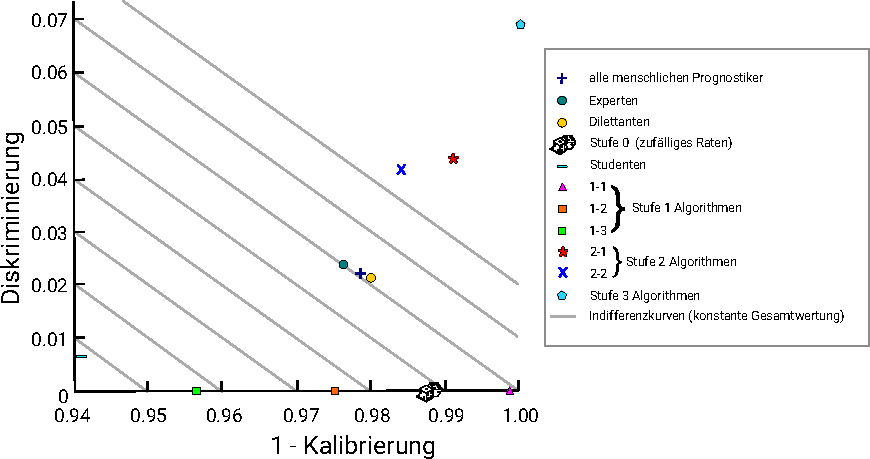
\includegraphics[scale=1.0]{Grafiken/Tetlock_1_Fertig_Ink.pdf} 
\label{pic:Tetlock_1}
\end{figure}
Die zwei
Bestandteile des \emph{probability score}, Kalibrierung (\emph{calibration}) und
Diskriminierung (\emph{discrimination}), sind auf den Achsen abgebildet. \\ \\ 
Kalibrierung (horizontale Achse) misst die Fähigkeit eines Prognostikers,
Ereignisse korrekt nach ihrer
Auftrittswahrscheinlichkeit zu ordnen (vgl. \cite{Tetlock}, S.~47). So ist ein
Prognostiker gut kalibriert, wenn etwa 10~\% der Ereignisse eintreten, für die
er eine Wahrscheinlichkeit von 0.1 geschätzt hat, 20~\% der Ereignisse eintreten
die eine Wahrscheinlichkeit von 0.2 erhalten haben, und so weiter. Je kleiner
der numerische Wert der Kalibrierung, desto besser ist der Prognostiker. Bei
einem Wert von 0 ist die bestmögliche Kalibrierung erreicht und aus diesem Grund
ist (1 - Kalibrierung) auf der horizontalen Achse abgebildet. \\ \\
Weiterhin ist ein Prognostiker umso besser bei der Diskriminierungskomponente
(vertikale Achse),
je eher es ihm gelingt die Auftrittswahrscheinlichkeiten von einzelnen
Ereignissen von der relativen Häufigkeit aller Ereignisse\footnote{
genauer: Das Verhältnis der Anzahl der eingetretenen Ereignisse zu der
Gesamtanzahl der Ereignisse} (\emph{base-rate})
zu unterscheiden. Perfekte Diskriminierung wird erreicht, wenn allen 
eingetretenen Ereignissen eine Wahrscheinlichkeit von 1.0 zugeordnet wird, und
alle Ereignisse, die nicht eingetreten sind, mit Null bewertet werden
(vgl. \cite{Tetlock}, S.~47).\\ \\
Nun gehen Kalibrierung und Diskriminierung als Summe in den
\emph{probability score} ein. Aus diesem Grund kann sich für verschiedene
Werte von Kalibrierung und Diskriminierung der gleiche Wert für den
\emph{probability score} ergeben. Die diagonalen Linien in Abbildung~\xcom
markieren Stellen mit konstantem \emph{probability score}. Je weiter rechts oben
eine Linie verläuft, desto höher ist der zugehörige \emph{probability score}.
\\ \\
Die Gesamtergebnisse für Kalibrierung und Diskriminierung für die verschiedenen
Teilnehmergruppen sind in der Graphik eingetragen. Die am besten qualifizierte
Gruppe stellen die Experten dar, die Fragen zu ihren jeweiligen Fachgebieten
erhalten haben (vgl. \cite{Tetlock}, S.~242). Weniger qualifiziert sind die 
\glqq{Dilettanten}\grqq (\emph{dilettantes}), Experten, die jedoch Fragen
beantwortet haben, die nicht zu ihrem Spezialgebiet gehören. Die Dilettanten
gaben an, dass sie sich mit Hilfe qualititativ hochwertiger Quellen
(\emph{Economist}, \emph{Wall Street Journal}, \emph{New York Times} etc.) über
Themen außerhalb ihrer Fachgebiete informieren (vgl. \cite{Tetlock}, S.~56).
Die Gruppe mit der geringsten Qualifikation waren Studenten, die die Übungen
zu Vorhersagen absolvieren mussten, nachdem sie kurze Zusammenfassungen von
Fakten zu den jeweiligen Themen erhalten haben (vgl. \cite{Tetlock}, S.~56).
\\ \\
Weiterhin enthält Abbildung~\ref{pic:Tetlock_1} auch die Ergebnisse, die von den
statistischen Algorithmen erzielt wurden. Zur besseren Übersicht werden die
Algorithmen hier in vier Gruppen eingeteilt. Der Stufe 0 Algorithmus würfelt
einfach die Antworten , er ordnet den zur Debatte stehenden Ereignissen
zufällige Wahrscheinlichkeiten zu. Weiterhin gibt es mehrere Varianten von
Stufe 1 Algorithmen, die als Antwort auf die Fragen immer die relative
Häufigkeit der Ereignisse eintragen. Etwas komplexer sind die Stufe 2
Algorithmen. Diese extrapolieren aus der Vergangenheit in die Zukunft und setzen
die Wahrscheinlichkeiten für die Ereignisse entsprechend. Die höchste
Komplexität hat der Stufe 3 Algorithmus. Um die Eintrittswahrscheinlichkeiten
der Ereignisse zu ermitteln, nutzt dieser die Vergangenheitswerte mehrerer
Variablen, die eine hohe Vorhersagekraft besitzen.\footnote{Die genaue Zuordnung
der Stufen 0-3 zu den Algorithmen in der Originalquelle (\cite{Tetlock}, S.~51)
sieht folgendermaßen aus:
\begin{description}
\item[Stufe 0:] \emph{random guessing} (\emph{chimp})
\item[Stufe 1:] \emph{contemporary base rate} (1-1), \emph{restrictive base
  rate} (1-2), \emph{expansive base rate} (1-3)
\item[Stufe 2:] \emph{cautious case-specific extrapolation} (2-1),
  \emph{aggressive case-specific extrapolation} (2-2)
\item[Stufe 3:] \emph{autoregressive distributed lag models}
\end{description}
} \\ \\
Abbildung~\ref{pic:Tetlock_1} zeigt, dass die Experten die Studenten bei
den \emph{forecasting exercises} deutlich schlagen konnten. Allerdings waren die
Experten kaum besser (!) als der zufallsgesteuerte Algorithmus 
(Stufe 0)\footnote{Die Experten waren schlechter kalibriert aber besser bei
der Diskriminierung, sodass sie insgesamt eine etwas bessere Gesamtwertung
hatten}. Insbesondere verloren die Experten gegen die komplexeren Algorithmen
(Stufe 2 und 3) mit deutlichem Abstand und zwar sowohl bei Kalibrierung, als
auch bei Diskriminierung. Falsche Überzeugungen und mentale Barrieren haben, so
Tetlock, das Urteilsvermögen der Experten getrübt und zu den schlechten
Ergebnissen geführt (mehr dazu in Abschnitt~\xcom). \\ \\
Was haben diese Ergebnisse mit \emph{predictive analytics} und dem öffentlichen
Sektor zu tun?\\ \\
Erstens waren die Fragestellungen der \emph{forecasting exercises} aus den
Bereichen Politik und Wirtschaft\footnote{
Andere Themen, wie beispielweise naturwissenschaftliche Fragestellungen,
z. B. \glqq{Wie} wahrscheinlich ist die Detektion dunkler Materie
in den nächsten fünf Jahren?\grqq, wurden nicht behandelt.
}, was für den öffentlichen Sektor relevant ist. Zweitens handelt es sich dabei
um generelle Probleme der menschlichen Urteilsfindung. Probleme, die in vielen
Bereichen auftreten und zu Fehleinschätzungen führen können. Zudem
konnten datenbasierte Algorithmen, also \emph{predictive analytics}, die
menschlichen Vorhersagen bei den \emph{forecasting exercises} schlagen. Dies
deutet darauf hin, dass formale Methoden wie \emph{predictive analytics} dabei
helfen können, bessere Urteile zu fällen und folglich auch bessere
Entscheidungen zu treffen. \\ \\
Der nächste Teil der Arbeit behandelt \emph{predictive analytics},
den Prozess der (menschlichen) Urteilsfindung und wie formale Methoden diesen
Prozess verbessern können.


\chapter{Konzepte von Predictive Analytics}
\label{part:Konzepte_PA}

\section{Begriffsdefinition und -Abgrenzung}

Das primäre Ziel von \emph{\gls{glos:Predictive_Analytics}} ist das Treffen von
Vorhersagen.
Hierbei sind nicht nur Prognosen für die Zukunft gemeint, sondern
auch Einschätzungen und Beurteilungen unklarer Situationen, bei denen die für
die Entscheidungsfindung wichtigen Daten fehlen (vgl. \cite{Dinov}, S.~9~f.).
Hier sind einige Anwendungsbeispiele, die verdeutlichen, wie \emph{predictive
analytics} eingesetzt werden kann (vgl. \cite{Schmitz}):
\begin{description}
\item[Betrugserkennung (\emph{fraud detection}):] Geschäftsvorgänge werden
automatisch analysiert, in der Hoffnung, dass Unregelmäßigkeiten vom System
erkannt werden. Verdächtige Vorgänge können dann zum Beispiel einer manuellen
Prüfung unterzogen werden.
\item[Vorhersage von Wartungszeitpunkten (\emph{predictive maintenance}):]
Automatische Systeme schätzen die Ausfallwahrscheinlichkeit von Maschinen ein
und bestimmen den Zeitpunkt für die nächste Inspektion.
\item[Verringerung von Ausschuss (\emph{predictive quality}):]
Mit Hilfe von Sensordaten werden fehlerhafte Produkte im Produktionsprozess
erkannt und aussortiert.
\item[Erkennung von Kundenunzufriedenheit (\emph{churn management}):]
Muster in Daten, die auf Unzufriedenheit von Kunden deuten, automatisch erkennen
und rechtzeitig Gegenmaßnahmen versuchen.
\item[Verbesserung der Zahlungsmoral:]
Mit Hilfe von Vorhersagen die Randbedingungen verbessern, sodass Kunden
schneller Rechnungen begleichen.
\item[Bessere Kontrolle von Personalfluktuationen:]
Mitarbeiter, die bald einen Arbeitsplatzwechsel vollziehen könnten, mit Hilfe
von Vorhersagemodellen erkennen, um rechtzeitig darauf reagieren zu können.
\end{description}
\begin{figure}%[!hbt]
\centering
\caption{Erstellung von Vorhersagemodellen.}
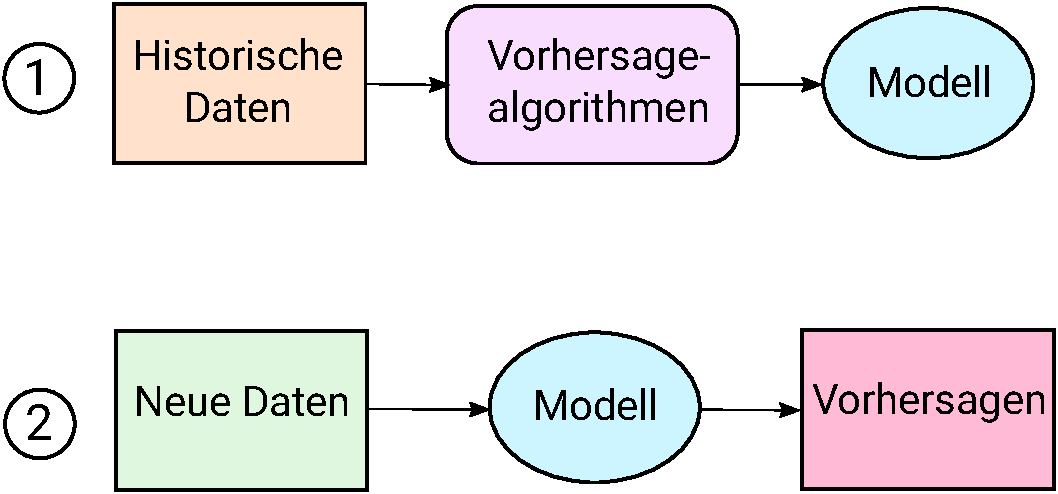
\includegraphics[scale=0.8]{Grafiken/PA_Ink.pdf} 
\label{pic:PA}
\end{figure}
Abbildung~\ref{pic:PA} veranschaulicht den allgemeinen Prozess zur Generierung
von Vorhersagemodellen\footnote{
Basierend auf dem Original aus \cite{Parthasarathy}.
}.
Zum Erstellen der Vorhersagen werden historische Daten benötigt. Diese Daten
werden von Algorithmen genutzt, um Modelle zu bauen. Die Vorhesagemodelle
akzeptieren neue Daten als Eingabe und liefern dazu eine Vorhesage der
gewünschten Eigenschaften. So könnte eine Versicherung beispielsweise
Vorhersagemodelle zur Betrugserkennung implementieren. Die historischen Daten
könnten in diesem Fall Forderungen von Kunden an die Versicherung aus der
Vergangenheit sein. Das Vorhesagemodell würde dann eine neue Forderung an die
Versicherung als Eingabe nehmen und könnte als Ausgabe eine Zahl zwischen 0 und
1 liefern. Dieser vorhergesagte Wert kann dann als Wahrscheinlichkeit
interpretiert werden, dass es sich bei der neuen Forderung um einen Betrugsfall
handelt. 


\section{Probleme menschlicher Urteile}

Die meisten Urteile und Prognosen werden von Menschen gefällt, ohne statistische
Modelle und Vorhersagealgorithmen zu nutzen. Grundsätzlich fällt jeder Mensch
Urteile, macht Vorhersagen und nutzt diese um Entscheidungen zu treffen. Aus
diesem Grund ist ein gutes Urteilsvermögen eine Eigenschaft, die eigentlich
universell gebraucht wird. Für die großen gesellschaftlichen Entscheidungen
versorgen Experten Wirtschaft, Politik und Öffentlichkeit mit Prognosen und
Einschätzungen. Dabei ist es üblich routinemäßig Expertenmeinungen einzuholen,
unüblich ist es allerdings, systematisch die Qualität dieser Urteile zu
überprüfen (vgl. \cite{Tetlock}, S.~1). Aus diesem Grund hat der Psychologe
Philip Tetlock sich zur Aufgabe gemacht, \glqq{gutes} Urteilsvermögen\grqq
formal fassbar zu machen (vgl. \cite{Tetlock}, S.~3). Nach Tetlock sollte gutes
Urteilsvermögen anhand zweier Kriterien gemessen werden (vgl. \cite{Tetlock},
S.~7):
\begin{description}
\item[(1) Richtigkeit der Vorhersagen (\emph{get it right}):]
\label{misc:Emp_Korr}
Empirische Korrespondenztests sollen genutzt werden, um zu überprüfen, wie gut
die Meinungen und Vorhersagen von Experten mit der Wirklichkeit übereinstimmen.
\item[(2) Logische Konsistenz des Denkmodells (\emph{think the right way}):]
Die Gedanken von Experten sollten logisch konsistent sein. Genauer ausgedrückt
bedeutet dies, dass die Denkmodelle nicht die Gesetze der Logik und der
Statistik missachten sollten. Zudem sollte eine Person mit einem guten
Urteilsvermögen ihre Glaubenssätze an neue Erkenntnisse anpassen können.
\end{description}
Dabei sollte die experimentelle Psychologie die notwendigen Fakten und
Einsichten liefern (vgl. \cite{Tetlock}, S.~8).

\subsection{Tetlocks Forecasting Exercises}

Für die empirischen Korresponenztests führten Tetlock und sein Team eine Reihe
von \emph{forecasting exercises} mit Experten durch. Diese Expertenbefragungen
wurden bereits in Teil~\ref{part:Schw_Vorhersagen} thematisiert und sollen nun
detaillierter erläutert werden. \\ \\
Insgesamt wurden die Urteile von 284 Experten analysiert. Diese hatten im
Durchschnitt 12 Jahre Berufserfahrung und die Hälfte (52~\%) besaß einen
Doktortitel. Etwa 61~\% der Teilnehmer wurden mindestens einmal von den Medien
interviewt und 21~\% mehr als zehnmal. Etwa 80~\% der Experten waren mindestens
einmal als Berater für internationale politische oder wirtschaftliche
Angelegenheiten tätig. (vgl. \cite{Tetlock}, S.~239-240)\\ \\
Die Befragten sollten Prognosen erstellen, indem sie auf Fragen zu zukünftigen
Entwicklungen in Politik und Wirtschaft antworteten. Dabei handelte es sich um
feste Fragestellungen, die von den Forschern zuvor ausgewählt wurden. Zu den in
den Fragen formulierten Szenarien sollten die Befragten subjektive
Wahrscheinlichkeiten\footnote{
Eine subjektive Wahrscheinlichkeit wird als Grad des Vertrauens einer Person in
den Eintritt eines Ereignisses interpretiert (vgl. \cite{Eisenfuehr}, S.~152).}
angeben. (vgl. \cite{Tetlock}, S.~245)\\ \\
Die Sammlung der Expertenprognosen begann 1987 und erstreckte sich über mehr als
zehn Jahre. Dabei wurden Fragen über die zukünftige Entwicklung von etwa 60
Nationen gestellt. (vgl. \cite{Tetlock}, S.~242)\\ \\
Weiterhin wurden die Fragen in folgende Themenbereiche untergliedert
(vgl. \cite{Tetlock}, S.~246-248):
\begin{description}
\item[(a)] Kontinuität politischer Führung
\item[(b)] Innen- und Wirtschaftspolitik
\item[(c)] Nationale Sicherheit und Verteidigungspolitik
\item[(d)] Zusätzliche Spezialthemen
\end{description}
Insgesamt wurden 82 361 subjektive Wahrscheinlichkeiten eingeholt, die als
Antwort auf circa 27 450 Fragen gegeben wurden. (vgl. \cite{Tetlock}, S.~246)

\subsection{Der Probability Score als Maß der Genauigkeit von Vorhersagen}

Die Fragen der \emph{forecasting exercises} wurden so formuliert, dass bei allen
nach einer gewissen Zeitspanne festgestellt werden konnte, ob und welches der
möglichen Szenarien\footnote{
Die möglichen Szenarien müssen dabei logisch vollständig sein und sich
gegenseitig ausschließen (\emph{logically exhaustive and mutually exclusive};
vgl. \cite{Tetlock}, S.~245).
} tatsächlich eingetreten ist. Um dann die, auf Seite~\pageref{misc:Emp_Korr}
erwähnte, Richtigkeit der Vorhersagen zu überprüfen, müssen die subjektiven
Wahrscheinlichkeiten mit der eingetretenen Wirklichkeit verglichen werden. \\ \\
Das Werkzeug zur Durchführung dieses Vergleichs und zur Bewertung der
Genauigkeit der erstellten Prognosen ist der \emph{probability score}\footnote{
  Auch \emph{Brier score} genannt (siehe \xcom)
} (vgl. \cite{Tetlock}, S.~46). Dabei werden die subjektiven
Wahrscheinlichkeiten (die Vorhersagen) mit den tatsächlich eingetretenen
Ereignissen (der Wirklichkeit) verrechnet\footnote{
  Es wird 0 eingesetzt, falls ein Szenario nicht eingetreten ist und 1 falls es
  eingetreten ist (vgl. \cite{Tetlock}, S.~46-47).
}. Das Ergebnis ist eine Zahl zwischen 0 und 1, wobei 0 die beste und 1 die
schlechteste Wertung darstellt. Wenn ein Prognostiker jedes Ereignis, das
schließlich eintritt, als unmöglich eingestuft hat und jedes Ereignis, welches
ausbleibt, als sicher, dann endet er beim schlechtesten \emph{probability
score} von 1. Die beste Wertung von 0 kann hingegen nur erreicht werden, indem
man, zumindest was die gestellten Fragen betrifft, hellseherische Fähigkeiten
beweist und jedes eingetretene Ereignis mit einer subjektiven Wahrscheinlichkeit
von 1 bewertet und jedem ausgebliebenen Ereignis eine 0 zugewiesen hat (vgl.
\cite{Tetlock}, S.~47). \\ \\
Zudem lässt sich der \emph{probability score} in zwei Komponenten zerlegen, die
von den Fähigkeiten des Prognostikers abhängen: Kalibrierung
(\emph{calibration}) und Diskriminierung (\emph{discrimination})\footnote{
  Die Bedeutung dieser beiden Komponenten wurde auch im einleitenden
  Teil~\ref{part:Schw_Vorhersagen} erläutert.
} (vgl. \cite{Tetlock}, S.~47). \\ \\
Die Kalibrierung misst wie gut ein Prognostiker
Ereignisse in Wahrscheinlichkeitskategorien einordnen kann\footnote{
  10~\% der Ereignisse aus der 0.1 Kategorie treten ein, 20~\% der Ereignisse
  aus der 0.2 Kategorie usw. 
}. Der Wertebereich der Kalibrierung liegt zwischen 0 und 1, wobei 0 den besten
und 1 den schlechtesten Wert darstellt (vgl. \cite{Tetlock}, S.~275). \\ \\
Die Diskriminierung misst wie gut sich die subjektiven Wahrscheinlichkeiten des 
Prognostikers von der relativen Häufigkeit (\emph{base-rate}) aller betrachteten
Ereignisse abheben. Der Wertebereich der Diskriminierung reicht von 0 bis zu
einem Wert, der die Unsicherheit der Umgebung, für die die Prognosen erstellt
werden, widerspiegelt (vgl. \cite{Tetlock}, S.~278). Im Falle der
Diskriminierung ist 0 der schlechteste Wert. Im besten Fall ist der Wert der
Diskriminierung gleich dem Wert der Unsicherheit. \\ \\
Die Kernidee bei der Anwendung des \emph{probability score} ist das Nutzen
des Gesetzes der großen Zahlen (\emph{law of large numbers})
(vgl. \cite{Tetlock}, S.~12-13). Einzelne Urteile mit subjektiven
Wahrscheinlichkeiten, die nicht 0 oder 1 sind, können nicht widerlegt werden,
da seltene Ereignisse eintreten können und häufige Ereignisse ausbleiben können.
Betrachtet man hingegen eine große Zahl an Vorhersagen, dann kann mit Hilfe
des \emph{probability score} die Genauigkeit des Prognostiker aus der Gesamtheit
seiner Vorhersagen eingeschätzt werden. \\ \\
Der Anhang~\xcom liefert die Formeln für den \emph{probability score}, wobei
dessen Berechnung zusätzlich anhand von Beispielen erläutert wird. \\ \\

\subsection{Detaillierte Ergebnisse der Forecasting Exercises}

Die Analyse der Ergebnisse der \emph{forecasting exercises} konnte Aufschluss
darüber geben, welche Attribute der Teilnehmer einen Einfluss auf die
Genauigkeit ihrer Vorhersagen haben und welche nicht. \\ \\
Zu den Attributen, die keinen Einfluss auf die Fähigkeiten der Experten haben,
gehören überraschenderweise (vgl. \cite{Tetlock}, S.~68):
\begin{itemize}
\item der Bildungsgrad (Doktortitel oder kein Doktortitel)
\item das Fachgebiet
\item die Erfahrung
\item der Zugang zu geheimen Informationen
\end{itemize}
Zudem hat Medienberühmtheit einen starken negativen Effekt auf die Fähigkeiten
der Prognostiker (vgl. \cite{Tetlock}, S.~68). \\ \\
Ein entscheidender Faktor, der gute von schlechte Prognostikern unterscheidet,
ist nicht ihr Weltbild, sondern ihre Art zu Denken (\emph{cognitive style})
(vgl. \cite{Tetlock}, S.~72 und S.~75). Tetlock unterteilt die Experten in
Abhängigkeit von ihrer Art zu Denken in Füchse (\emph{foxes}) und Igel
(\emph{hedgehogs})\footnote{
In Anlehnung an das Essay \emph{The Hedgehog and the Fox} des Philosophen Isaiah
Berlin.
}. Genauer ausgedrückt, ist das wichtigste Maß für den \emph{cognitive style}
eines Experten ein Wert auf einer kontinuierlichen Skala (vgl. \cite{Tetlock},
S.~87). An einem Ende der Skala befinden sich die \emph{foxes}, an dem anderen
die \emph{hedgehogs}. Dazwischen befinden sich die hybriden Ausprägungen
\emph{fox-hog} (eher \emph{fox} als \emph{hedgehog}) und \emph{hedge-fox} (eher
\emph{hedgehog} als \emph{fox}). Bestimmt wird der Wert als Ergebnis eines
Fragebogens (siehe \cite{Tetlock}, S.~241). Dabei ist der Punkt, der am
stärksten in die Gewichtung einfließt, die Frage nach der Selbstidentifikation
(vgl. \cite{Tetlock}, S.~74 Tabelle~3.3)\footnote{
Hierbei werden Gewichtungen angegeben, mit denen die einzelnen Fragen in
die Bewertung einfließen. Je höher der Betrag des Gewichts, desto stärkeren
Einfluss hat die Frage auf das Ergebnis. Das Vorzeichen des Gewichts gibt an,
in welche Richtung die jeweilige Frage das Ergebnis verschiebt. Ein negatives
Vorzeichen verschiebt den Wert auf der Skala in \emph{hedgehog} Richtung, ein
positives Vorzeichen hingegen in \emph{fox} Richtung.   
}. Diese Frage lautet übersetzt (siehe \cite{Tetlock}, S.~241):
\begin{quotation}
%\begin{spacing}{1.2}
Isaiah Berlin unterteilte Intellektuelle in Igel und Füchse. Der Igel kennt eine
große Sache und versucht so viel wie möglich innerhalb dieses konzeptionellen
Rahmens zu erklären, wohingegen der Fuchs viele kleine Dinge weiß und damit
zufrieden ist, von Fall zu Fall andere improvisierte Erklärungen zu
finden. Ich positioniere mich zum Igel- oder Fuchsende dieser Skala.
% Isaiah Berlin classified intellectuals as hedgehogs or
% foxes. The hedgehog knows one big thing and tries to explain as much as
% possible within that conceptual framework, whereas the fox knows
% many small things and is content to improvise explanations on a case-
% by-case basis. I place myself toward the hedgehog or fox end of this
% scale
%\end{spacing}
\end{quotation}
Abbildung~\ref{pic:Hedgehog_Fox} erläutert die Skala des \emph{cognitive style}.
\\ \\
\begin{figure}%[!hbt]
\centering
\caption{Skala des \emph{cognitive style}%, mit den Charakterisierungen
%  \emph{Fox} und \emph{Hedgehog} als Gegenpole}
}
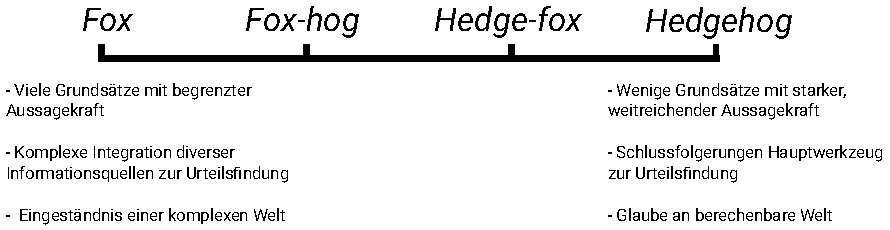
\includegraphics[scale=1]{Grafiken/Hedgehog_Fox.pdf} 
\label{pic:Hedgehog_Fox}
\end{figure}
\emph{Hedgehogs} haben einige wenige Glaubenssätze, die sie nutzen um
Erklärungen für die unterschiedlichsten Dinge abzuleiten (vgl. \cite{Tetlock},
S.~73). Sie bemühen sich, Fakten in Einklang mit ihren präferierten Grundsätzen
zu bringen und fällen ihre Urteile, indem sie Schlussfolgerungen aus einer
kleinen Menge an Überzeugungen ziehen. Zudem tendieren \emph{hedgehogs}
zu intellektuellem \glqq{Geiz}\grqq (\emph{parsimony}) (vgl.\cite{Tetlock}, 
S.~20). Dies bedeutet, dass sie nur ungerne neue Grundsätze
aufstellen und stattdessen versuchen, mit ihren wenigen, schon vorhandenen
Glaubenssätzen weitreichende Erklärungen für eine große Bandbreite an Phänomenen
zu erhalten. Zudem zeichnen sich \emph{hedgehogs} durch eine starke
Selbstsicherheit in Bezug auf die Genauigkeit ihrer Prognosen und Urteile aus
(vgl. \cite{Tetlock}, S.~73). \\ \\
\emph{Foxes} hingegen sind skeptisch bezüglich starker Glaubenssätze, die alles
umspannende Erklärungen liefern sollen. Stattdessen vertrauen sie auf viele
Grundsätze mit begrenzter Aussagekraft (\emph{tricks of their trade}) (vgl.
\cite{Tetlock}, S.~73). Weiterhin ist die Urteilsfindung bei \emph{foxes} keine
reine Übung in deduktiver Logik (vgl. \cite{Tetlock}, S.~73), sondern benötigt
die Integration diverser Informationsquellen. \emph{Foxes} sind eher zaghaft,
wenn es darum geht, ihre eigenen Fähigkeiten als Prognostiker zu loben (vgl.
\cite{Tetlock}, S.~73-74). \\ \\
\begin{figure}%[!hbt]
\centering
\caption{Leistungsunterschiede bei den \emph{forecasting exercises} in
  Abhängigkeit vom \emph{cognitive style} der Teilnehmer}
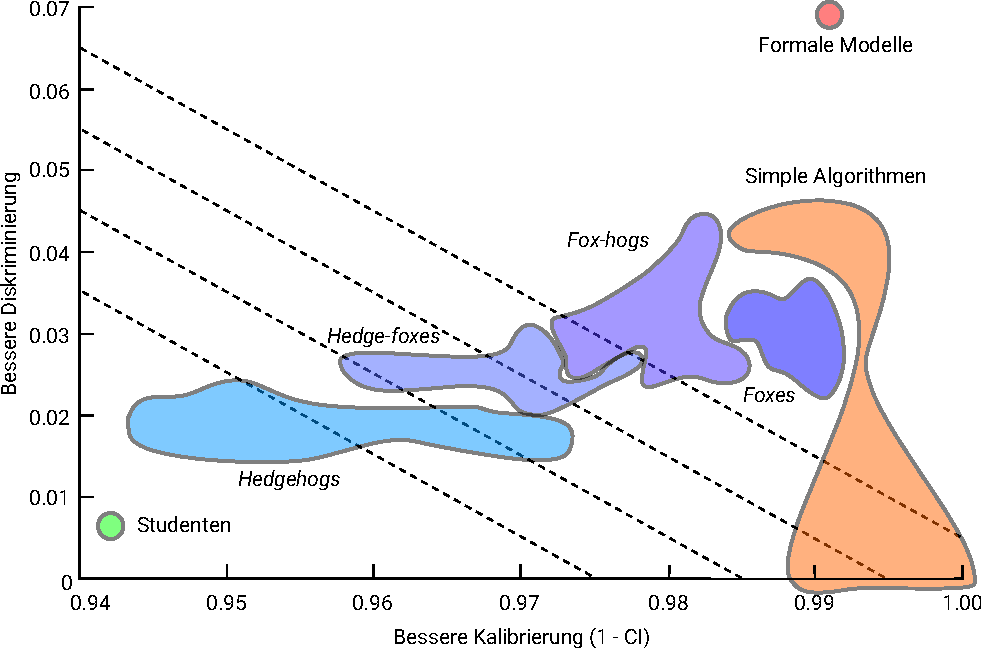
\includegraphics[scale=0.88]{Grafiken/Tetlock_2_Ink.pdf} 
\label{pic:Tetlock_2}
\end{figure}
Ein Ergebnis von Tetlocks \emph{forecasting exercises} wurde bereits in
Abbildung~\ref{pic:Tetlock_1} aus Teil~\ref{part:Schw_Vorhersagen} erläutert.
Dort war ersichtlich, dass die Experten im Vergleich zu statistischen
Algorithmen schlecht abschnitten. Abbildung~\ref{pic:Tetlock_2} zeigt nun ein
differenzierteres Bild von der Leistung der Experten.  
% Urteilskraft einzelner Experten bezüglich Kalibrierung und Diskriminierung
% variiert 
%\subsection{Analyse der Ergebnisse der Forecasting Exercises}

% (vgl. \cite{Tetlock}, S.~XXX)

% parsimony lohnt nicht (S. 68)
Tetlock ist der Meinung, dass die Kernaufgabe politischer Weltanschauungen
nicht die Erstellung möglichst korrekter Prognosen ist, sondern die
Aufrechterhaltung einer bequemen Illusion von Berechenbarkeit
(vgl. \cite{Tetlock}, S.~39). Somit sind die Ergebnisse schlecht, weil
nüchterner Realismus unerwünscht ist. Die Aufrechterhaltung von Glaubenssätzen,
die zum kollektiven Zusammenhalt beitragen, hat höhere Priorität.

Insgesamt wird die Befürchtung, dass sich Menschen durch Wunschdenken leiten
lassen (vgl. \cite{Eisenfuehr}, S.~181) und dass sie das oft tun, von Tetlocks
Arbeit bestätigt.


\begin{table}
\centering
\caption{Ausgewählte Beispiele für kognitive Verzerrungen}
\label{tab:Kognitive_Verzerrungen}
\scalebox{0.7}{
\begin{tabular}{ |l|l|l|  }
\hline
\textbf{Bezeichnung der kognitiven Verzerrung} & \textbf{Sinngemäße Übersetzung}
  & \textbf{Kurzbeschreibung} \\
\hline
{ \large \emph{Anchoring} } & Ankereffekt
  & Beharren auf einer ersten \\
& & Schätzung eines Wertes; \\
& & unzureichende Anpassung\\
& & nach weiterem Überlegen.\\
\hline
{ \large \emph{Attribution bias} } & Zuschreibungsfehler
  & Die Tendenz, Erfolge \\
& & seinen eigenen Fähigkeiten \\
& & zuzuschreiben; \\
& & Misserfolge hingegen \\
& & externen Zuständen. \\
\hline
{ \large \emph{Availability bias} } & Verfügbarkeitsfehler
  & Beispiele für Szenarien, \\
& & die unmittelbar mit einem \\
& & Ereignis assoziiert werden, \\
& & bestimmen die Einschätzung \\
& & dieses Ereignisses. \\
\hline
{ \large \emph{Base rate neglect} } & Vernachlässigung von Basisraten
  & Vernachlässigung allgemeiner \\
& & Wahrscheinlichkeiten und \\
& & Konzentration auf fallspezifische \\
& & Informationen. \\
\hline
{ \large \emph{Cognitive conservatism} } & Kognitiver Konservatismus
  & Weigerung von Menschen, \\
& & Fehler zuzugeben und \\
& & ihre Meinung zu ändern. \\
\hline
{ \large \emph{Gambler's fallacy} } & Irrtum des Glücksspielers
  & Der irrtümliche Glaube an \\
& & regelmäßige Muster \\ 
& & in zufälligen Prozessen. \\
\hline
{ \large \emph{Hindsight bias} } & Rückschaufehler
  & Der Versuch eine Einschätzung \\
& & eines Ereignisses, nach dessen \\
& & Eintreten, rückwirkend zu \\
& & verändern. \\
\hline
{ \large \emph{Overconfidence effect} } & Selbstüberschätzung
  & Überschätzung der Richtigkeit \\
& & eigener Urteile. \\
\hline
\end{tabular}
}
\end{table}

\subsection{Auswirkungen von Tetlocks Forschungsergebnissen}

\section{Bestandteile von \emph{predictive analytics}}

Bei \emph{predictive analytics} werden Daten mit Hilfe von geeigneten Methoden
verarbeitet, um verschiedene Arten von Prognosen zu ermöglichen. Dem
Datenanalysten stehen für diese Aufgabe Computeranwendungen zur Verfügung.
Diese Programme lesen die Daten ein, führen die notwendigen Berechnungen aus und
ermöglichen eine graphische Aufbereitung der Ergebnisse. \\ \\
Standardisierte
Vorgehensmodelle können helfen, die Arbeitsschritte einer Datenanalyse zu
vereinheitlichen. Ein Beispiel für ein solches Vorgehensmodell ist CRISP-DM \xcom.

\subsection{CRISP-DM Vorgehensmodell}

\subsection{Daten}

\subsubsection{Elementare Datentypen}

Bei Daten lassen sich verschiedene elementare Typen\footnote{Alternativ dazu
spricht man vom Skalenniveau (\emph{scale of measurement}) als eine
Eigenschaft von Daten und Variablen.} unterscheiden.
Je nach Datentyp einer
Variablen, werden ihre Werte unterschiedlich interpretiert. Zudem können
bestimmte mathematische Operationen nur mit Variablen eines bestimmten Typs
durchgeführt werden. Die Datentypen werden im folgenden Text genauer erläutert
(vgl. \cite{Arens}, S.~1229 und \cite{McCarthy}, S.~28-29).\\ \\
Der \glqq{einfachste}\grqq Datentyp ist eine nominal skalierte Variable. 
Werte von nominal skalierten Variablen werden als Namen
interpretiert. Weiterhin ist es nicht sinnvoll diese Art von Variablen zu
ordnen. Es lässt sich lediglich feststellen, ob zwei Variablen
gleich oder ungleich sind. Ein Beispiel für eine nominal skalierte Variable ist
der Name einer Stadt. Die Werte sind dann konkrete Städtenamen wie
\glqq{München}\grqq oder \glqq{Berlin}\grqq. Als Operationen stehen nur $=$
oder $\neq$ zur Verfügung, weil Aussagen wie 
\glqq{München}\grqq$=$\glqq{München}\grqq oder
\glqq{München}\grqq$\neq$\glqq{Berlin}\grqq sinnvoll sind. Nicht sinnvoll wären
dagegen Vergleiche wie \glqq{München}\grqq$<$\glqq{Berlin}\grqq
\footnote{Der Vergleich wäre sinnvoll, wenn mit der Nennung des Namens 
z. B. implizit die Größe der Stadt gemeint wäre. Dies ist hier aber nicht der
Fall.}.
Weitere Beispiele für nominal skalierte Variablen sind Geschlecht, Augenfarbe
oder Postleitzahl. \\ \\
Etwas mehr Möglichkeiten stehen zur Verfügung, wenn eine ordinal skalierte
Variable vorliegt. Für eine solche Variable ist eine Ordnung sinnvoll, sodass
alle Vergleichsoperationen möglich sind. Eine Kleidungsgröße (\texttt{S},
\texttt{M}, \texttt{L}) ist ein Beispiel für eine ordinal skalierte
Variable. Im Gegensatz zum Beispiel mit den Städtenamen ist ein Vergleich wie
\texttt{S} $<$ \texttt{M} hier sinnvoll. \\ \\
Wird eine Variable auf einer Intervallskala definiert, sind ihre Werte
numerisch.
Zusätzlich zu
allen Operationen von nominal und ordinal skalierten Variablen können hier auch
Additionen und Subtraktionen ausgeführt werden. Ein Beispiel hierfür sind
Temperaturen in °C, die addiert und subtrahiert werden können. Allerdings sind
20~°C nicht das Doppelte von 10~°C. Hier kann man erkennen, dass es bei
Intervallskalen nicht sinnvoll ist, Verhältnisse zu berechnen. Der Grund
hierfür ist, dass der Nullpunkt einer Intervallskala nicht mit dem absoluten
Nullpunkt einer Größe identisch sein muss. So sind 0~°C nicht der absolute
Nullpunkt für die Temperatur. Wenn man sinnvolle Verhältnisse berechnen will,
wird eine Proportionalskala benötigt. \\ \\
Eine auf einer Proportionalskala definierte Variable hat numerische Werte, für
die alle zuvor erwähnten mathematischen Operationen definiert sind und
zusätzlich auch Multiplikation und Division möglich sind.
%Insbesondere ist es sinnvoll Verhältnisse zu berechnen.
So führt eine
Multiplikation einer Länge in Metern mit der Konstante 2 zu der doppelten Länge.
Ist das Verhältnis zweier Längen gleich 10, so ist die eine Länge 10
mal so groß wie die andere. Weiterhin führt die Multiplikation zweier Längen
in m zu einer korrekten Fläche in $\textrm{m}^2$. Die Ergebnisse wären nicht
korrekt, wenn der Nullpunkt der Meterskala nicht mit dem Nullpunkt der
Längenskala identisch wäre, wie es bei Intervallskalen der Fall ist. \\ \\
Nominal und ordinal skalierte Variablen sind qualitative Variablen.
Variablen, die auf Intervall- oder Proportionalskalen definiert sind, werden
hingegen als quantitative oder kardinale Variablen bezeichnet.
Weiterhin werden qualitative Variablen auch als kategorisch
(\emph{categorical}) bezeichnet, quantitative als numerisch (\emph{numeric})
und je nach Wertebereich als diskret (\emph{discrete}, ganzzahlige Werte) oder
kontinuierlich (\emph{continuous}, Fließkommawerte). \\ \\
Tabelle~\ref{tab:Skalen} zeigt eine Zusammenfassung der verschiedenen Datentypen
und der erlaubten Operationen\footnote{
Basierend auf Tabelle 2.2 in \cite{Runkler}, S.~8}.
\begin{table}
%\footnotesize
\centering
\caption{Übersicht der Datenskalen}
\label{tab:Skalen}
\scalebox{0.7}{
\begin{tabular}{ |l|l|l|l|  }
\hline
\textbf{Skala} & \textbf{Sinnvolle Operationen}
  & \textbf{Beispielgrößen} & \textbf{Beispielwerte} \\
\hline
Nominal & Gleichheit ($=, \neq$) & Name, & \glqq{Julia}\grqq,
  \glqq{Klaus}\grqq \\
& & Geschlecht & \texttt{M}, \texttt{W} \\
\hline
Ordinal & Gleichheit ($=, \neq$), & Kleidungsgröße & \texttt{S}, \texttt{M},
  \texttt{L} \\
        & Vergleiche ($<, >, \ldots$) & & \\
\hline
Intervall & Gleichheit ($=, \neq$), & Jahresangabe, & 2015~n.Chr. \\
  & Vergleiche ($<, >, \ldots$), & Temperatur in Grad Celsius & 20~°C \\
  & Addition ($+$), Subtraktion ($-$), &  &  \\
\hline
Proportional & Gleichheit ($=, \neq$), & Alter, & 21 Jahre \\
  & Vergleiche ($<, >, \ldots$), & Temperatur in Kelvin & 273.4~K \\
  & Addition ($+$), Subtraktion ($-$), &  &  \\
  & Multiplikation ($\cdot$), Division ($/$) & & \\
\hline
\end{tabular}
}
\end{table}


\subsubsection{Information Management (Data Warehouse)}

\subsubsection{Datenabhängige Ziele}

\paragraph{\ldots}

\paragraph{Beschreibung der Daten}

\paragraph{Klassifikation}

\paragraph{Zeitreihenanalyse}

\subsection{Methoden}

\begin{figure}%[!hbt]
\centering
\caption{\emph{Predictive analytics} Methoden aus der Anwenderperspektive.}
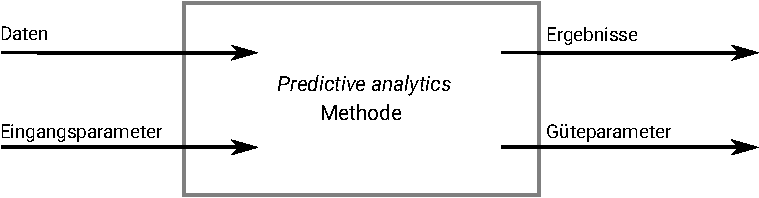
\includegraphics[scale=1.0]{Grafiken/PA_Methoden_Ink.pdf} 
\label{pic:PA_Methoden}
\end{figure}

\subsubsection{Die Großen Drei}

\paragraph{Regression}

\paragraph{Entscheidungsbäume}

\paragraph{Neuronale Netze}

\subsubsection{Zeitreihenanalyse}

\subsubsection{\ldots}

\subsection{Werkzeuge}

\subsection{(Kreative) Freiheitsgrade bei der Implementierung eines
  Vorhersagemodells}

\section{Anwendungsbeispiele}

\subsection{Allgemeine Anwendungsfelder (siehe SAP Artikel)}

\subsection{\ldots}

\section{Allgemeine Risiken bei der Nutzung von Predictive Analytics}

Es existieren Risiken, die dazu führen können, dass die Ziele einer
Datenanalyse nicht oder nicht in vollem Umfang erreicht werden können.
Im folgenden Text werden einige dieser Risiken erläutert.

\subsection{Risiko der Unverhältnismäßigkeit}

Die Anwendung von Predictive Analytics ist mit einem hohen Aufwand verbunden.
Dabei spielen die Kosten für die Datenerhebung eine wesentliche Rolle.
Zusätzlich werden für die Datenanalyse Kenntnisse aus verschiedenen
Fachrichtungen benötigt. So sind einerseits anwendungsspezifische Kenntnisse
zur Interpretation der Daten und der Ergebnisse wünschenswert. Andererseits
werden zur Durchführung der Datenanalyse Kenntnisse in Mathematik, Statistik und
Informatik benötigt. \\ \\
Aus diesem Grund besteht das Risiko, dass die Kosten einer Anwendung von
Predictive Analytics den Nutzen übersteigen. Es ist auch möglich, dass das
gleiche Ergebnis mit einer einfacheren, kostengünstigeren Methode erreicht
werden kann. In diesem Fall würde die Anwendung eines aufwändigen Predictive
Analytics Verfahrens wertvolle Ressourcen binden, die an anderer Stelle stärker
gebraucht werden. \\ \\
Somit ist es wichtig, Betrachtungen zu Alternativkosten \todo{gls eintrag}
in die Planung von \emph{predictive analytics} Anwendungen einzubeziehen. 

\subsection{Risiken bei der Datenerhebung}

Trainingsdaten spiegeln nicht (mehr) das Verhalten des Systems wider.

\subsubsection{\ldots}

\subsection{Risiken bei der Interpretation der Daten}

\subsection{Risiken bei der Interpretation der Ergebnisse}

Wenn die Ergebnisse der Datenanalyse zur Entscheidungsunterstützung herangezogen
werden, beeinflussen sie das Verhalten der Entscheidungsträger. Dies kann zur
Entstehung problematischer psychosozialer Effekte führen. Zwei Beispiele hierfür
werden nun erläutert.

\subsubsection{Prognose verändert das Verhalten des Systems }

Die Ergebnisse von Vorhersagen werden von Menschen interpretiert,
die daraufhin ihr Verhalten anpassen. Dies kann zu Rückkopplungseffekten führen,
die von negativen Auswirkungen im Sinne einer
\glqq{Selffulfilling} Prophecy\grqq begleitet werden können
(vgl. \cite{Crossman}). Bestimmte Prognosen können beispielsweise von einer 
Interessengruppe als Bestätigung ihrer Agenda interpretiert werden, wobei
anders lautende Vorhersagen ignoriert werden. Dadurch bestärkt, setzt die Gruppe
ihre gewünschten Handlungsoptionen um. Dies ruft den vorhergesagten Effekt
jedoch erst hervor.

\subsubsection{Ignorieren der Unsicherheiten bei der Prognose}

Es besteht die Gefahr, dass die Unsicherheiten von Vorhersagen ignoriert werden
und die Prognose als eine Gewissheit betrachtet wird. Somit wird möglichen,
alternativen Entwicklungen bei der Entscheidungsfindung nicht genügend Bedeutung
beigemessen. Dies kann dazu führen, dass Risiken falsch kalkuliert werden und
in der Zukunft nicht genügend Handlungsoptionen zur Verfügung stehen.


\chapter{Predictive Analytics im öffentlichen Sektor}

% TODO
% Stand Entscheidungshilfen (wie vorstellbar: Mensch entscheidet, Computer
%   unterstützt)
% Abgrenzung zum privaten Sektor
% auf operativer Ebene allerdings ähnlich
% unterschied strategisch, taktische Ebene, operativ
% top management, mittleres management, operatives management 
% s. Watson, Abschnitt Lack of regulation and algorithm bias
% TODO bias insgesamt (in Rahmenbedingungen)
\begin{figure}%[!hbt]
\centering
\caption{Risikomatrix für die Nutzung maschineller Entscheidungshilfen}
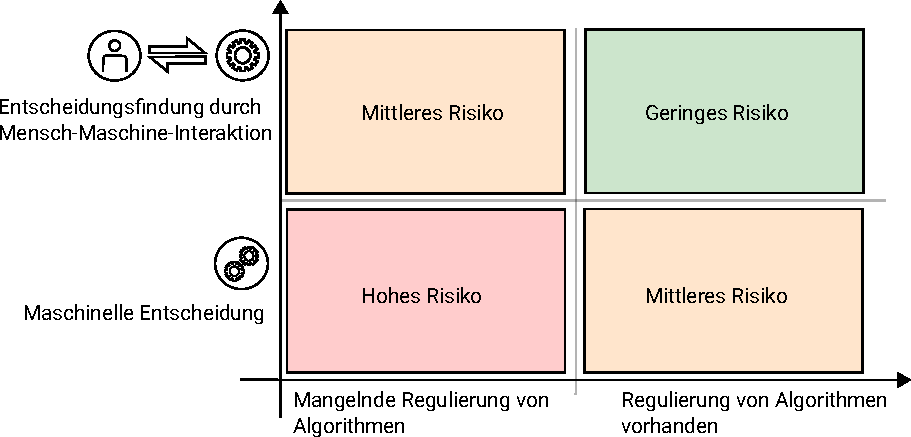
\includegraphics[scale=1.0]{Grafiken/Risk_Matrix_Ink.pdf} 
\label{pic:Risiko_Matrix}
\end{figure}

\section{Rahmenbedingungen}

% TODO Technologie prinzipiell kein Hindernis (s. IT Novum)

% TODO
% Politiker, Experten und Kommentatoren formulieren keine subjektiven Wsk und
% niemand berechnet den Brier Score (oder ein anderes Maß)
% Widerstände auf strat und takt Ebene gegen Forecasting und PA
% Forecasting und PA nicht auf dem Vormarsch
% Forecasting leichter zu sehen,
% PA auf operativer Ebene (Tabellenkalkulation) verschleiert Widerstand auf
% takt und strategischer Ebene (!)
% Rahmenbedingungen:
% - Wahrheit taktisch genutzt
% - versch. Gruppen/Kulturen -> versch. Wahrheiten
% - Themen kontroverser (vs. z. B. Fruchtsäfte)
% - Konkurrenz (v. a. bei strategischen Entscheidungen) 
% - Ignorieren (-> Probleme menschl. Urteile)

%-------------------------------------------------------------------------------
Tetlock ist der Meinung, dass die Kernaufgabe politischer Weltanschauungen
nicht die Erstellung möglichst korrekter Prognosen ist, sondern die
Aufrechterhaltung einer bequemen Illusion von Berechenbarkeit
(vgl. \cite{Tetlock}, S.~39). Somit sind die Ergebnisse schlecht, weil keine
genaue Abbildung der Realität beabsichtigt wird. Die Aufrechterhaltung von
Glaubenssätzen, die zum kollektiven Zusammenhalt beitragen, hat höhere
Priorität.

In diesem Zusammenhang sind auch verschiedene Interpretationen des
Wahrheitsbegriffs bedeutsam. Eine weit verbreitete Interpretation wird mit
Hilfe des Pragmatismus von William James definiert. Demnach werden
Aussagen von Menschen als Wahrheit akzeptiert, falls die Aussagen ihnen bei der
Orientierung in der Welt nützlich sind. Dies liefert eine Erklärung dafür, dass
Menschen dazu tendieren Aussagen zu glauben, die ihre eigene Weltsicht
bestätigen. Bei einer extremen Ausprägung des pragmatischen Wahrheitsbegriffs
wird aus der Nützlichkeit einer Aussage ihr Wahrheitsgehalt abgeleitet:
\glqq{Es ist wahr, weil es nützlich ist}\grqq. (vgl. \cite{Precht})

Diese radikale Wahrheitsinterpretation ist problematisch, wenn die als Wahrheit
betrachteten Grundsätze der Realität widersprechen. Denn es gibt keine
Möglichkeit, die Grundsätze mit Hilfe von empirischen oder logischen Beweisen
zu revidieren und an die Realität anzupassen. Langfristig führen falsche
Grundsätze somit zu schlechtem Urteilsvermögen, was wiederum zu schlechten
Entscheidungen führt. Insbesondere sind Datenanalysen in einer solchen Situation
nicht zweckdienlich, da Ergebnisse selektiv ignoriert oder abgelehnt werden.

Eine andere Interpretation von Wahrheit legt großen Wert auf die Beweisbarkeit
von Aussagen. Eine solche Interpretation ist beispielsweise in der Wissenschaft
verbreitet. Aussagen wird erst dann ein Wahrheitswert zugewiesen, wenn
unwiderlegbare Beweise für die Gültigkeit der Aussage vorhanden sind. Eine
solche Interpretation weicht stark vom pragmatischen Standpunkt ab, kann aber
ebenfalls problematisch werden. Es besteht die Gefahr sich bei der Prüfung von
Aussagen in Kleinigkeiten zu verlieren, handlungsunfähig zu werden oder
nützliche Erkenntnisse zu lange anzuzweifeln\footnote{
Beispiele für Zweifel, die gefährlich werden, weil sie Fortschritt blockieren
sind auf Seite~\xcom erläutert.
}.

Vermutlich ist für ein gutes Urteilsvermögen ein nüchterner Pragmatismus
notwendig, bei dem vorsichtig zwischen Nutzen und Wahrheit abgewogen wird und
auch unangenehme Meinungen als Wahrheit akzeptiert werden können.
Bedauerlicherweise gerät ein solcher Pragmatismus mit jeder, insbesondere
politischen, Weltanschauung in Konflikt, die selbst nicht in ähnlicher Weise
pragmatisch ist.

%-------------------------------------------------------------------------------

\subsection{Eine pessimistische Sichtweise}

Je mehr das Treffen von Entscheidungen zur Hauptaufgabe von Personen gehört,
desto stärker betrachten sie \emph{predictive analytics} als eine Gefahr für
ihren Arbeitsplatz.

Es gibt Stimmen, die behaupten, dass ein immenser Widerstand gegen die
Einführung solcher Methoden [Forecasting + Predictive Analytics] zu erwarten
ist. Teilweise deutet sich sogar eine Unmöglichkeit dieser Aufgabe an. Beim 
Thema Forecasting ist es Tetlock selbst, der sich skeptisch äußert. Er
benennt den Widerstand der Experten als die größte Barriere zur Einführung der
neuen Methodik (\emph{the most daunting of all the barriers to implementation},
vgl. \cite{Tetlock}, S.~235). Jackson und Reichin vertreten eine ähnliche
Auffassung (vgl. \cite{Jackson}, S.~295).

Der investigative Charakter von Datenanalysen kann Nervosität und Unbehagen
auslösen.

% TODO Daten (-> Heise) 
% Thapa_Parycek S. 46
\subsection{Eine optimistische Sichtweise}

% Formalisierung erwünscht (BBC + IC)

Bessere Prognosen und Urteile führen zu besseren Entscheidungen. Dies bringt
wiederum sowohl Vorteile gegenüber Konkurrenten als auch Vorteile bei der
Auseinandersetzung mit der \glqq{Natur}\grqq\footnote{
Genauer: Bei der Auseinandersetzung mit den Zwängen, die durch die Naturgesetze
und ökonomische Prinzipien definiert werden. Verzichtet man zum Beispiel auf das 
Rauchen kann es als eine gute Entscheidung betrachtet werden, da man dadurch
gesünder lebt. Hierfür muss zunächst erkannt werden, dass Rauchen ungesund ist.
Klingt heute einfach. Diese Erkenntnis zu erlangen war jedoch mit erheblichem
Aufwand verbunden, wobei auch wissenschaftliche und statistische Methoden
eine große Rolle spielten (vgl. zum Beispiel \cite{Proctor}).

Ein weiteres Beispiel für eine Entscheidung, die nicht in erster Linie Vorteile
gegenüber Konkurrenten verspricht, ist eine Entscheidung für eine bessere
Behandlungsmethode in der Medizin. Denn der primäre Zweck davon ist, die 
Möglichkeit zu erlangen, mehr Menschen zu heilen.
}

\section{Spieltheoretische Betrachtung}

Aufgrund der potentiell konfliktreichen Situation rund um die Einführung von
\emph{forecasting} oder \emph{predictive analytics}, bietet es sich an, die
\gls{glos:Spieltheorie} anzuwenden.

\subsection{Einleitung zur Spieltheorie}
% TODO


% deadlock (S. 218(
\begin{figure}%[!hbt]
\centering
\caption{Deadlock Auszahlungsmatrix}
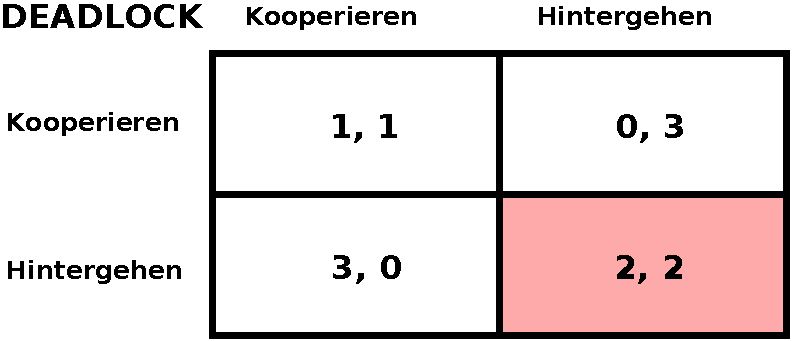
\includegraphics[scale=0.8]{Grafiken/Deadlock_Ink.pdf} 
\label{pic:Deadlock}
\end{figure}

% stag hunt (S. 220)
\begin{figure}%[!hbt]
\centering
\caption{Stag Hunt Auszahlungsmatrix}
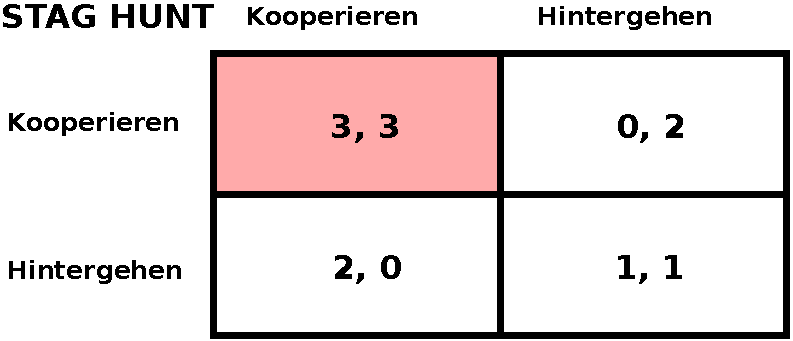
\includegraphics[scale=0.8]{Grafiken/Stag_Hunt_Ink.pdf} 
\label{pic:StagHunt}
\end{figure}

% mixed
\begin{figure}%[!hbt]
\centering
\caption{Gemischte 'Stag Hunt - Deadlock' Auszahlungsmatrix}
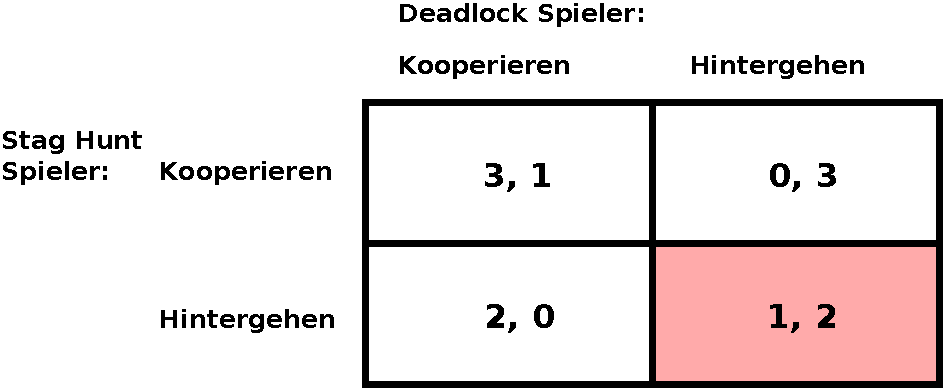
\includegraphics[scale=0.7]{Grafiken/Mixed_Ink.pdf} 
\label{pic:Mixed}
\end{figure}

\subsection{Kritische Würdigung der spieltheoretischen Betrachtung}

% TODO spielen implizit spieltheorie (s. Poundstone ?)

% prisoners dilemma (S.237)
% mixed
\begin{figure}%[!hbt]
\centering
\caption{Gefangenendilemma Auszahlungsmatrix}
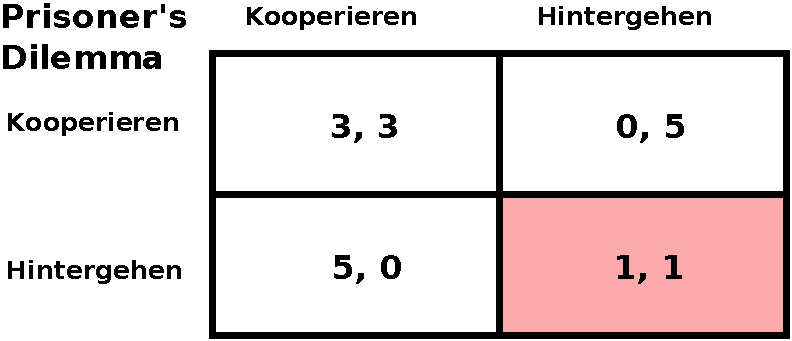
\includegraphics[scale=0.8]{Grafiken/Prisoner_Ink.pdf} 
\label{pic:Prisoner}
\end{figure}

\chapter{Anwendungen von Predictive Analytics im öffentlichen Sektor}

Zum Schluss werden einige Anwendungen von Predictive Analytics im öffentlichen
Sektor vorgestellt. Es wurden Anwendungsfälle in den Bereichen öffentliche Verwaltung,
Gesundheit und Bildung betrachtet. Zudem wurden Fallstudien erstellt, bei denen
konkrete Anwendungen im Fokus stehen.

% TODO
% 2 grundlegende Probleme
% - Datenschutz: Achtung Privatsphäre + Angst vor Missbrauch
% - Verzerrungen in Daten: insb. auch Big Data, Daten nicht repräsentativ,
%     Daten kulturabhängig

\section{Öffentliche Verwaltung}


\subsection{Open Data Portale}

Open Data Portale veröffentlichen Daten von Behörden, sodass prinzipiell jeder
sie nutzen kann. So existiert in den USA beispielsweise das Portal \glqq{Data.gov}\grqq{}\footnote{
URL für das US-Portal: \url{https://www.data.gov/}
}, das deutsche Pendant dazu heißt \glqq{GovData.de}\grqq{}\footnote{
URL für die deutsche Version: \url{https://www.govdata.de/} 
} (vgl. \cite{Borchers}). 

Grundsätzlich könnten die Daten auch für Predictive Analytics Zwecke genutzt werden.
Allerdings hat eine stichprobenartige Untersuchung ergeben, dass es sich bei vielen Daten
nicht mehr um \glqq{Rohdaten}\grqq{} handelt, sondern um eine aufbereitete Fassung, die sich
für die visuelle Präsentation eignet. Für Datenanalysen wären jedoch die Rohdaten besser geeignet.
Weiterhin scheinen manche Behörden im Vergleich zu anderen viele Daten an das Portal zu übergeben,
sodass die Auswahl dann unausgeglichen wirkt. Zudem gibt es die Kritik, dass viele relevante
Datensätze nicht veröffentlicht werden (vgl. \cite{Krempl}).

% TODO Daten (-> Heise) 
% Thapa_Parycek S. 46

Insgesamt ist aus der stichprobenartigen Untersuchung der Datensätze auf GovData.de nicht unmittelbar
hervorgegangen, wie die Daten für Predictive Analytics Anwendungen sinnvoll eingesetzt werden könnten. 

\subsection{Predictive Analytics in der Steuerverwaltung}

Die Anwendungen von Predictive Analytics in der Steuerverwaltung werden in einer
Studie des \emph{Forum on Tax Administration} (FTA) diskutiert\footnote{
Deutschland ist bei dieser Studie allerdings nicht dabei.
}. Der folgende Text beschreibt diese Anwendungsfälle.

\subsubsection{Audit Case Selection}

Steuerbehörden führen Kontrollen von Unternehmen und Personen durch, um Steuerbetrug
aufzudecken und zu verringern. Um verfügbare Ressourcen besser einzusetzen, werden mit Hilfe
von Predictive Analytics die Fälle für die Prüfung priorisiert, bei denen der größte Betrugsverdacht
besteht (Risikogruppen). Dieser Prozess wird als \emph{Audit Case Selection} bezeichnet und ist das hauptsächliche
Anwendungsgebiet von Predictive Analytics in der Steuerverwaltung (vgl. \cite{OECD}, S.~20).

Eine Besonderheit dabei ist die Analyse sozialer Netzwerke (\emph{Social Network Analysis}; \cite{OECD}, S.~21-22),
die zur Aufdeckung besonderer Formen von Einkommenssteuerbetrug eingesetzt wird. Die Analyse sozialer Netzwerke kann
Risikogruppen finden, die von Analysen auf individueller Ebene übersehen werden. Bei der Analyse werden die Beziehungen
zwischen Individuen erkennbar und können als visualisierte Netzwerke betrachtet werden. Die weitere Analyse dieser Netzwerke
kann durch Sachbearbeiter erfolgen oder mit Hilfe von regelbasierten oder statistischen Modellen durchgeführt werden.

\subsubsection{Payment Compliance}

Das Ziel der Payment Compliance ist es, ausstehende Zahlungen möglichst einzufordern oder das Problem gar nicht erst
entstehen zu lassen (vgl. \cite{OECD}, S.~24). Die typische Aufgabe von Predictive Analytics ist hierbei, die
Steuerzahler herauszufiltern, bei denen das größte Risiko besteht, dass sie ihre Zahlungsverpflichtungen nicht erfüllen werden. 
Eine weitere Anwendung, ist herauszufinden, wie am effektivsten mit dieser Gruppe kommuniziert werden kann (Prescriptive Analytics).

\subsubsection{Debt Management}

Beim traditionellen Debt Management werden Gruppen von Hochrisikoschuldnern identifiziert, um vorhandene Ressourcen auf sie zu
konzentrieren (vgl. \cite{OECD}, S.~26). Bei einer neueren Methode (\emph{Uplift Modelling}) werden Fälle selektiert, die
mit möglichst hoher Wahrscheinlichkeit auf eine Intervention seitens der Behörde reagieren werden. 

\subsubsection{Verbesserung der Serviceleistungen für Steuerzahler}

Text Mining (inklusive \emph{Sentiment Analysis}) kommt bei den Steuerbehörden zum Einsatz, um die Kommunikation mit den
Steuerzahlern zu verbessern (vgl. \cite{OECD}, S.~27). So werden beispielsweise ankommende E-Mails in Singapur mit Hilfe
von Text Mining bearbeitet, um die Art der Anfrage herauszufinden (vgl. \cite{OECD}, S.~27-28). In einem Fall konnte eine
Gruppe ähnlicher Anfragen identifiziert werden, nachdem eine Steuerrichtlinie verändert worden war. Die Behörde war dann in
der Lage frühzeitig zu reagieren und die Steuerzahler zusätzlich zu informieren. Text Mining hat in Singapur die manuelle
Bearbeitung von E-Mail Anfragen abgelöst. Dies ermöglicht eine objektivere Verarbeitung der Anfragen, da weniger Missverständnisse
entstehen. Zusätzlich wird die Arbeitszeit der Sachbearbeiter eingespart.

\subsubsection{Entscheidungsunterstützung}

Die meisten Datenanalysen bei den Steuerbehörden werden durchgeführt, um operative
Entscheidungen zu unterstützen (vgl. \cite{OECD}, S.~28). Allerdings exisitieren auch
Anwendungen, die strategische und politische Entscheidungen unterstützen. So werden
Analysen zur Abschätzung der Steuerlücke (\emph{tax gap analysis};vgl. \cite{OECD}, S.~28) durchgeführt.
Weiterhin wird versucht, den Einfluss von Änderungen in der Steuerpolitik vorherzusagen. Ein Beispiel
dafür, wenn auch streng genommen keine Predictive Analytics Anwendung, ist das ökonomische Modell, das
2012 von den chinesischen Behörden erstellt wurde, um die Effekte einer Steuerreform auf die Wirtschaft
und die soziale Wohlfahrt abzuschätzen (vgl. \cite{OECD}, S.~29). Der entsprechende Bericht der
Datenanalysten spielte eine wichtige Rolle in dem folgenden Reformprozess.

\subsubsection{Probleme mit Daten}

Der Bericht des FTA enthält auch eine Diskussion einiger Probleme, die im Zusammenhang mit Daten
festgestellt wurden.

So gibt es Bedenken, ob die gesammelten Daten, die anschließend für das Training der Modelle verwendet werden,
repräsentativ sind (vgl. \cite{OECD}, S.~51). Denn die verwendeten Daten stammen oft von stark verzerrten
Stichproben, wie beispielsweise alten Untersuchungsfällen. Somit wird nur ein kleiner Ausschnitt aus der
Gesamtpopulation zum Training der Modelle verwendet, was zu Selektionseffekten und schließlich zu Verzerrungen
im Modell führt. Um dieses Problem zu beheben, beziehen US-Steuerbehörden ihre Daten aus zufällig ausgewählten
Stichproben von Steuerprüfungen, um die Daten repräsentativer zu gestalten (vgl. \cite{OECD}, S.~52).

Weiterhin werden die Daten für Predictive Analytics Projekte eigentlich für operative Zwecke erhoben und
gespeichert (vgl. \cite{OECD}, S.~52). Aus diesem Grund ergeben sich verpasste Gelegenheiten, denn manche Daten, die nicht sinnvoll
für operative Zwecke sind, können nützlich für Datenanalysen sein. Zum Beispiel werden Beanstandungsgründe nach
einer Steuerprüfung typischerweise nicht gespeichert. Diese Information wäre jedoch hilfreich, um gesonderte Modelle
für verschiedene Beanstandungsgründe zu erstellen (vgl. \cite{OECD}, S.~52). 

\subsection{Predictive Policing}

Predictive Policing bezeichnet die Erstellung von Datenanalysen, um Verbrechen zu verhindern, Verbrechensfälle zu lösen
und wahrscheinliche Ziele für Polizeieinsätze zu identifizieren (vgl. \cite{Perry}, S.~1-2). Dabei können diese Methoden
in folgende vier Kategorien eingeteilt werden (vgl. \cite{Perry}, S.~8-9):

\begin{description}

\item[(1) Vorhersage von Verbrechen:] \hfill \\
Bei diesen Methoden sollen Plätze und Zeiträume identifiziert werden,
bei denen das Risiko für Verbrechen besonders hoch ist.

\item[(2) Vorhersage von Kriminellen:] \hfill \\
Hierbei sollen einzelne Personen identifiziert werden, die ein Risiko
tragen, in Zukunft Verbrechen zu begehen.

\item[(3) Vorhersage von Täterprofilen:] \hfill \\
Diese Methoden sollen Täterprofile generieren, die begangene Verbrechen
den wahrscheinlichen Tätern zuordnen.

\item[(4) Vorhersage der Opfer von Kriminalität:] \hfill \\
Hierbei sollen bestimmte Gruppen oder Einzelpersonen identifiziert werden,
bei denen ein erhöhtes Risiko besteht, Opfer von Verbrechen zu werden.

\end{description} 

\begin{figure}%[!hbt]
\centering
\caption{Predictive Policing Prozess}
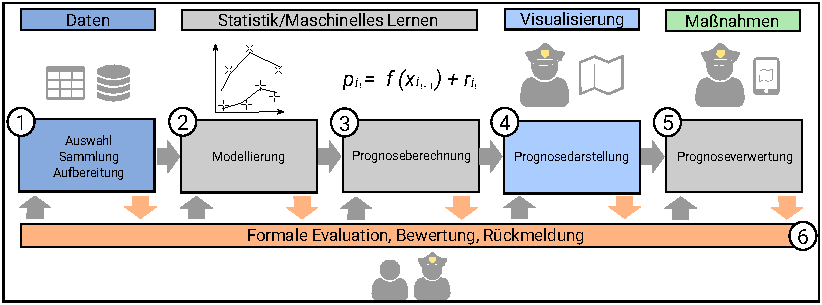
\includegraphics[scale=1.1]{Grafiken/Predictive_Policing_Ink.pdf} 
\label{pic:Predictive_Policing}
\end{figure}

In Deutschland werden bisher nur die Methoden von Punkt (1) verwendet, mit denen
Delikte wie Wohnungseinbrüche behandelt werden (vgl. \cite{Heuberger}).
Abbildung~\ref{pic:Predictive_Policing} zeigt hierbei das Vorgehen\footnote{
Das Original ist in \cite{Bode}, S.~2 zu finden.
}. Dies ist ähnlich zu den
allgemeinen Vorgehensmodellen aus Abschnitt~\xcom. Insbesondere die anwendungstypischen Details werden
im folgenden Text erläutert:

\begin{description}

\item[(1) Daten:] \hfill \\
Hierbei können polizeiliche und nicht-polizeiliche Daten kombiniert werden. Weiterhin
besteht die Notwendigkeit, die verschiedenen Daten korrekt zusammenzuführen, damit beispielsweise die räumliche
und zeitliche Konsistenz gewährleistet ist (vgl. \cite{Bode}, S.~2). Zudem werden bisher keine
personenbezogenen Daten verwendet (vgl. \cite{Bode}, S.~2 und \cite{Heuberger}) und die Daten konzentrieren
sich auf Wohnungseinbruchdiebstahl (vgl. \cite{Bode}, S.~2)

\item[(2) Modellierung:] \hfill \\
Für die Modellierung können die üblichen Algorithmen wie Regression, Entscheidungsbäume oder
neuronale Netze verwendet werden (vgl. \cite{Bode}, S.~2).

\item[(3) Prognoseberechnung:] \hfill \\
Das Ergebnis der Prognose ist eine Menge an Gebieten, die für den betrachteten Zeitraum
ein höheres Kriminalitätsrisiko aufweisen (vgl. \cite{Bode}, S.~2).

\item[(4) Prognosedarstellung:] \hfill \\
Neben der altmodischen Variante von Karten im Papierformat, existieren auch graphische
Visualisierungen mit Hilfe von Tablet-PCs oder Mobilfunkgeräten (vgl. \cite{Bode}, S.~3).

\item[(5) Prognoseverwertung:] \hfill \\
Die Prognosen werden durch operative Polizeieinheiten genutzt, die ihre Aktionen mit Hilfe
der Vorhersagen planen können (vgl. \cite{Bode}, S.~2).

\item[(6) Evaluation:] \hfill \\
Während das System arbeitet erfolgt auch immer wieder eine Bewertung der Leistung des Systems.
Die Evaluation beeinflusst die Schritte (1)-(5) (vgl. \cite{Bode}, S.~3).

\end{description}

\subsubsection{Bisheriges Fazit von Predictive Policing in Deutschland}

Bereits im RAND Bericht von 2013 wurde betont, dass Computer nicht von alleine die Probleme
lösen können. Es braucht viel Arbeit und Korrektureingriffe von Menschen (vgl. \cite{Perry}, S.~117-118). 
Dies ist sowohl auf datenanalytischer Ebene der Fall, als auch auf der sozialen Ebene, auf der
\glqq{Feldarbeit}\grqq{} notwendig ist, um das Wissen über die konkrete Kriminalitätsumgebung auf dem
neuesten Stand zu halten. 

Das Fazit von Predictive Policing in Deutschland ist bisher gemischt. Es gibt Berichte über hohe
Trefferquoten der Anwendungen. Diese sollten allerdings mit Skepsis beurteilt
werden, da bei der Berechnung der Trefferquoten mangels konkreter Regelungen Abweichungen
entstehen können (vgl. \cite{Bode}, S.~9).
Diese Unregelmäßigkeiten können in folgenden Bereichen entstehen (vgl. \cite{Bode}, S.~9-11):

\begin{description}
\item[Prognose-Delikt:] Welches Art des Delikts wurde konkret vorhergesagt?
\item[Prognose-Dauer:] Für welchen Zeitraum wurde die Prognose angefertigt?
\item[Prognose-Raum:] Zählen Treffer an Gebietsrändern?
\end{description}

Weiterhin kam ein Evaluationsbericht für die Anwendung des Predictive Policing Werkzeugs PRECOBS
zu dem Schluss, dass es schwer zu beurteilen ist, ob die Anwendung zu einer Verminderung von
Wohnungseinbrüchen geführt hat, und dass das Werkzeug wahrscheinlich nur zu einer moderaten Kriminalitätsminderung
beigetragen hat (vgl. \cite{Gerstner}, S.~85).  

\subsection{Wahlen und Politik}

Neben den in Abschnitt~\xcom erwähnten Text Mining Anwendungen zur Verbesserung der Serviceleistungen
von Behörden existieren noch weitere \glqq{experimentelle}\grqq{} Anwendungen. So konnte Matter durch
die Analyse teilstrukturierter Internetdokumente herausfinden, wie stark öffentliche Ämter in den USA
mit religiösen Personen besetzt sind (vgl. \cite{Matter}). Der \glqq{Bible Belt}\grqq{}\footnote{
Der \glqq{Bible Belt} ist eine besonders religiöse Region der USA, die sich über mehrere Bundesstaaten erstreckt.
} und der Mormonenstaat Utah waren deutlich als relgiös konservative Staaten erkennbar (vgl. \cite{Matter}, S.~1078).
Weiterhin konnten Falck et al. die weltanschauliche Nähe von Zeitungen zu politischen Parteien und einzelnen Politikern
darstellen, indem sie die Einstellungen der Zeitschriften zu den jeweiligen Personen und Parteien analysierten
(\emph{sentiment analysis}; vgl. \cite{Falck}, S.~4). Somit können mit Hilfe von Text Mining die weltanschaulichen Präferenzen
von Personen und Organisationen bestimmt werden. Allerdings ist der praktische Nutzen solcher Analysen (noch) nicht klar.
Personen, die sich mit Politik beschäftigen, können solche weltanschaulichen Differenzen mit Hilfe ihrer Erfahrung relativ
schnell einschätzen.

In den USA werden Datenanalysen bei Wahlkämpfen verwendet. So waren im Wahlkampfteam von
Hillary Clinton im Jahr 2016 mehr als 60 Mathematiker und Datenanalysten beschäftigt (vgl. \cite{Goldmacher}). 
Die Modelle, die sie anwenden, dienen unter anderem dazu, \glqq{Wackelkandidaten}\grqq{} unter Delegierten zu identifizieren,
um die verfügbaren Ressourcen an Wahlwerbung auf sie zu fokussieren (vgl. \cite{Goldmacher}). Allerdings hat Donald Trump bei der damaligen Wahl
fast nichts in Datenanalysen investiert (vgl. \cite{Goldmacher}) und trotzdem gewonnen.

Ein bekannteres (und umstritteneres) Beispiel für die Anwendung von Datenanalysen
für politische und wahlkampftaktische Ziele ist der Fall von Cambridge Analytica.

\subsubsection{Cambridge Analytica - Fallstudie}

\begin{figure}%[!hbt]
\centering
\caption{Nutzung von Facebook Likes zur Vorhersage von Nutzerattributen}
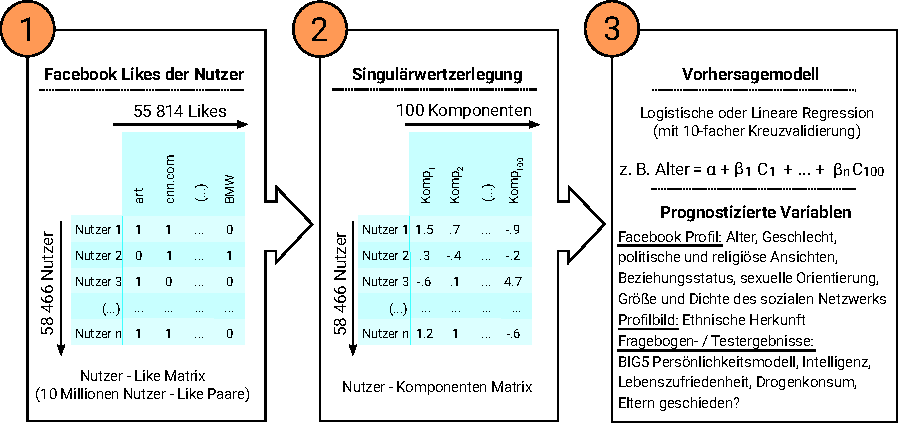
\includegraphics[scale=1.0]{Grafiken/Facebook_Likes_Ink.pdf} 
\label{pic:Like_Matrix}
\end{figure}

Den Grundstein für die Tätigkeit von \emph{Cambridge Analytica} hat ein Artikel
von Forschern der Cambridge Universität gelegt\footnote{
Genauer: Forscher vom \emph{Psychometrics Centre} in Cambridge
} (\cite{Kosinski}). Diese haben Persönlichkeitsmerkmale und Eigenschaften von
Personen vorhergesagt, indem sie die Nutzung von \emph{Facebook Likes} analysierten.
Abbildung~\ref{pic:Like_Matrix} veranschaulicht dieses Vorgehen\footnote{
Für die Orignalgrafik siehe \cite{Kosinski}, S.~5803.
}. Die Facebook Likes (Variablen) von tausenden Nutzern wurden mit Hilfe einer Methode zur
Variablenreduktion\footnote{
Die Singulärwertzerlegung ist eine Methode, die ähnlich zur Principal Component Analysis ist.
} auf 100 Komponenten verkleinert. Diese Komponenten dienten anschließend als Prädiktorvariablen
für die Vorhersagemodelle. Das Alter wurde beispielsweise mit linearer Regression bestimmt.
Die Modell konnte mit Hilfe der Informationen aus dem Facebook Profil, dem
Profilbild und der Ergebnisse eines psychologischen Tests trainiert werden (Trainingsdatensatz).
Das Ergebnis der Studie war, dass die Persönlichkeitsmerkmale und Attribute von Personen mit hoher
Genauigkeit von den Modellen vorhergesagt werden konnten\footnote{
Manche Attribute,wie z. B. das Alter, konnten genauer vorhergesagt werden als andere Merkmale, wie z. B. die Lebenszufriedenheit (vgl. \cite{Kosinski}, S.~5804)
} (vgl. \cite{Kosinski}, S.~5804).

Es wird vermutet, dass die Forscher aus Cambridge oder die Universität selbst sich geweigert haben, diese Nutzerdaten
preiszugeben (vgl. \cite{Isaak}, S.~57). Eine andere Forschergruppe hat in Kooperation mit Cambridge Analytica die
erforderlichen Daten mit Hilfe einer Umfrage von Facebook Nutzern gesammelt und dabei durch die Freigiebigkeit der Schnittstelle von
Facebook auch gleich die Daten der Freunde der Befragten erhalten (vgl. \cite{Isaak}, S.~57).

Das Ziel von Cambridge Analytica war es, mit dem Prognosemodell bestimmte Wählergruppen zu identifizieren (vgl. \cite{Isaak}, S.~57).
Diese würden dann im Laufe von Wahlen gezielt Nachrichten erhalten (Mikrotargeting). Dabei sollten entweder Wähler davon abgehalten
werden für den Konkurrenten zu stimmen, oder Wähler dazu verleitet werden für den gewünschten Kandidaten zu stimmen.

Die Einschätzungen über die Effektivität solcher Mikrotargeting Methoden gehen weit auseinander. So schreibt Trump in einem
Artikel der \emph{Washington Post} unter anderem, dass es sehr schwer sei mit Hilfe vom Mikrotargeting die politischen Ansichten
einer Person zu beeinflussen (vgl. \cite{Trump}). Außerdem hätten andere Mikrotargeting Kampagnen in der Vergangenheit keinen
eindeutigen Nutzen gezeigt. Andere Stimmen behaupten, dass die Arbeit von Cambridge Analytica einen nützlichen oder sogar
kritischen Effekt auf den Wahlausgang von 2016 hatte (vgl. \cite{Isaak}, S.~58).

Christliche Vereinigungen in den USA nutzen ähnliche Methoden, mit dem Ziel neue Mitglieder für die Kirche
zu gewinnen (vgl. \cite{Viken}, Minuten 13-19). So ist beispielsweise \emph{Gloo} eine christliche Softwarefirma,
die sich auf die Verknüpfung von Datenbanken spezialisiert hat. Gloo vermarktet seine Mikrotargeting Plattform
\emph{Insights} an Kirchen, wobei auch Daten der Kirchenmitglieder erfasst werden. Ein Werbespot für Insights
wirbt damit, ihren Kunden eine \glqq{Rundumansicht ihrer Zielgruppe in einer geschützten Datenbank mit mehr als 
2200 Datenpunkten zu nahezu jedem US Verbraucher}\grqq{} (siehe \cite{Viken}) zu bieten. Matt Engel, ein Gloo
Mitarbeiter, meint dass Gloo die größte Datenplattform mit missionarischem Ziel weltweit aufgebaut habe (vgl. \cite{Viken}).

Ein Geldgeber und Untestützer von Gloo beschreibt in einem Szenario, wie die Methode von Insights funktioniert (vgl. \cite{Viken}).
Die Anwendung identifiziert eine Zielgruppe von etwa 5 000 bis 10 000 Personen in einem Umkreis von etwa 15~km um eine Kirche.
Aus den Daten zu den Einkäufen der Personen kann geschlossen werden, ob manche Paare vielleicht Eheprobleme haben.
Diese Personen werden dann ausgewählt und die Anwendung hilft der Gemeinde, Kontakt mit ihnen über Facebook herzustellen.
Von der Kirche werden dann gezielt Einladungen zu Treffen, wie beispielsweise Abendveranstaltungen, verschickt. Wenn das Ehepaar
Kinder hat, werden sie während der Veranstaltung kostenlos betreut. Die neuen Kirchenbesucher können dann Kontakte mit
Mitgliedern aus der Kirchengemeinde knüpfen und möglicherweise selbst beitreten oder sich in Zukunft stärker engagieren.
Wie bereits oben erwähnt, dient die Methode also dazu, alte Mitglieder zu halten und neue für die Kirche zu gewinnen,
und somit die Kirchengemeinde zu vergrößern.

Einschätzungen dazu, wie effektiv das christliche Mikrotargeting funktioniert, wurden allerdings nicht gegeben.

\section{Gesundheit}

Schon seit dem letzten Jahrhundert können statistische Methoden von Wissenschaftlern
genutzt werden, um Gefahren für die öffentliche Gesundheit zu untersuchen (vgl. \cite{Proctor}, S.~216).

Allerdings hat sich dadurch auch das Phänomen der \glqq{Evidenzbeharrlichkeit}\grqq{} in der Epidemiologie etabliert
(vgl. \cite{Proctor}, S.~112-113).
Epidemiologen beharren auf strenger Evidenz und großen Fallzahlen (vgl. \cite{Proctor}, S.~112-113) und ignorieren weniger 
starke Indizien, wodurch der Fortschritt manchmal blockiert wird. Dies war bei der Anerkennung der Gesundheitsgefahren
von Asbest der Fall (vgl. \cite{Proctor}, S.~112-113). Im Jahr 1938 lag die Zahl der bekannten Krebserkankungen im Zusammenhang mit
Asbest weltweit bei 6. Somit konnten Epidemiologen behaupten, dass die Fallzahl nicht reiche, um einen signifikanten Zusammenhang
zwischen Asbest und Lungenkrebs herzustellen. Die Beweiskraft einer klinischen Studie, die den Zusammenhang hergestellt hat, indem sie
zwei Einzelfälle untersucht hat, galt als zu schwach (vgl. \cite{Proctor}, S.~113). Somit wurde die krebserregende Wirkung von Asbest
in Großbritannien und den Vereinigten Staaten nicht in den frühen 1940er Jahren sondern mehr als 20 Jahre danach anerkannt.

Die Geschichte scheint sich während der COVID-19 Pandemie wiederholt zu haben. Es wurde damit gehadert, Ergebnisse von Studien anzuerkennen,
die behaupteten, dass einfache Masken das Infektionsrisiko senken, weil sie nicht die strengen Kriterien der evidenzbasierten Medizin
entsprachen (vgl. \cite{Jotten}). Somit wurde das Tragen von Masken anfangs nicht vom Robert-Koch-Insitut empfohlen.

\subsection{Datenschutzbedenken}
% TODO Datenquellen

Das Thema Datenschutz bestimmt in Deutschland die Diskussion von Datenanalysen
im Gesundheitssektor (vgl. \cite{Jorzig}, S.~138-139 und \cite{Weichert}, S.~835-836 und \cite{Moebus}, S.~903). 
Insbesondere der Grundsatz der Datensparsamkeit, wozu Datenvermeidung, Datenlöschung und das Prinzip der Nichtverkettbarkeit gehören,
steht im Gegensatz zu den Bedürfnissen von des Big Data Konzepts, das durch Anhäufung und Verknüpfung vieler Daten Erkenntnisgewinne
sucht (vgl. \cite{Weichert}, S.~836). Aus diesem Grund müssen Gesundheitsdaten entweder annonymisiert oder pseudonymisiert werden:

\begin{description}

\item[Anonymisierung:] \hfill \\
Bei der Anonymisierung der Daten darf die Reidentifizierung nicht mehr erfolgen können.
Somit müssen bei Patientendaten nicht nur die Identifikationsmerkmale der Patienten entfernt werden, sondern
auch die Identifikatoren sämtlicher Dienstleister, die eine Zuordnung des Patienten vornehmen könnten,
entfernt werden (vgl. \cite{Weichert}, S.~836). Zu solchen Dienstleistern zählen beipielsweise Ärzte oder Apotheker.
Zusätzlich muss für eine vollständige Anonymisierung eine Aggregierung der Daten erfolgen, wobei z. B. Individualdatensätze
zu Gruppendatensätzen zusammengefasst werden, was allerdings die Datenqualität senkt (vgl. \cite{Weichert}, S.~836).

\item[Pseudonymisierung:] \hfill \\
Eine weitere Möglichkeit, die Daten datenschutzrechtlich nutzbar zu machen, ist die Pseudonymisierung.
Dabei werden die Identifikationsmerkmale von Patienten durch Kennzeichen ersetzt, was die Wiederzuordnung der Daten
erschweren soll (vgl. \cite{Weichert}, S.~836). Die Auswertung der pseudonymisierten Daten muss dann in einer geschützen
Umgebung erfolgen, die die Wiederzuordnung der Daten ausschließen soll (vgl. \cite{Weichert}, S.~837).
Dieser Ansatz wird auch als \emph{Differential Privacy} bezeichnet (vgl. \cite{Jorzig}, S.~140-141).

\end{description}

Hierbei sei jedoch erwähnt, dass die Datenschutzgrundverordnung, Datenanalysen zu wissenschaftlichen Zwecken erlaubt
(vgl. \cite{Jorzig}, S.~139). Dies wird als Forschungsprivileg bezeichnet. Allerdings sind müssen die oben genannten
strengen Einschränkungen beachtet werden.

\subsection{}




% Computertomographie 111-112
Buch: \cite{Jorzig}

Dud: \cite{Weichert}



% TODO Missbrauch -> Proctor



\subsection{Seuchenerkennung mit AI}
% TODO
% Google Flu Trends (vorerst gescheitert)

% TODO
%\subsection{Flint Trinkwasserskandal - Fallstudie}

\section{Bildung}
Abschließend sollen noch die Anwendungsmöglichkeiten von Predictive Analytics
im Bildungssektor kurz skizziert werden.

Eine weitere Anwendung ist E$^2$Coach, ein System zur Studienunterstützung.

\subsection{University of Michigan E$^2$Coach - Fallstudie}

E$^2$Coach wurde an der Universität von Michigan entwickelt (vgl. \cite{Mattingly}, S.~242).
Der Zweck der Einführung von E$^2$Coach war eine Verringerung der Abbrecherquoten in den
MINT-Fächern zu erreichen. Als historische Daten dienten dabei die Studienverlaufsdaten von
49 000 Studienanfängern im Fach Physik. Aus diesen Daten wurde ein Modell generiert.
Risikostudenten können mit Hilfe dieses Modells identifiziert werden, indem ihre Daten in das
System eingegeben werden. Dabei liefern Tutoren, Physikprofessoren und die Studenten selbst
die individuellen Daten der Studenten.

Um Feedback für die Studenten zu ermöglichen, agiert E$^2$Coach als Schnittstelle zwischen
den Studenten und den Ressourcen, die ihnen zur Verfügung stehen (z. B. Online Lernmaterial) (vgl. \cite{Mattingly}, S.~242).
So bietet das System den Studenten Fortschrittsanzeigen, Vorschläge für Lernmethoden und Ermutigungen.
Zudem gibt es menschliche Berater, die mit den Studenten über eine Online-Plattform kommunizieren können.
Bei den Beratern handelt es sich um Tutoren, die bereits einen Studienabschluss besitzen und die auf Basis
gemeinsamer Ziele und Interessen den zu beratenden Studenten zugewiesen werden.

Anwendungen wie E$^2$Coach, wären womöglich auch in Deutschland denkbar, falls die Nutzung personenbezogener
Daten auf Freiwilligkeit basiert.

Insgesamt scheint der Bildungssektor bisher am wenigsten von
Predictive Analytics Anwendungen profitiert zu haben.

% konkreteres Anwendungsbeispiel Decision Tree

%-------------------------------------------------------------------------------

% TODO echten Titel ersinnen
%\chapter{Zusammenfassung und Fazit}

% Grad der Etablierung von Forecasting kann ein Indikator für eine mögliche erfolgreiche Adoption
% von PA sein

% TODO Interessantes
% inwiefern lassen sich kognitive Verzerrungen vermeiden (s. Anhang für
%   ein Paar Betrachtungen hierzu)


%%%%%%%%%%%%%%%%%%%%%%%%%%%%%%%%%%%%%%%%%%%%%%%%%%%%%%%%%%%%%%%%%%%%%%%%%%%%%%%%
\appendix

% TODO evtl umbennen 
\chapter{Forecasting - Technische Details}


% TODO
% Brier Score Erklärung
% Brier Score Probleme
%   Vorhersage unwahrscheinlicher Ereignisse nicht gewürdigt
%   50/50 fence sitters -> unbefriedigend, Frustration (need for closure, S. 81)
%   % S. 276 Indiscriminate fence-sitting
% Bayes Belief Updating Erklärung/Herleitung
% Kognitive Verzerrungen, Auflistung, Diskussion
%   Erlernbar oder nicht (- individuell nicht gelungen, + in Gruppe, 
%     Kommunikation hilft, Unterschiede nicht unüberwindbar)
% + eher statistisch, mathematische "Verzerrungen" (subadditivity ...)
% 11 Commandments GJP



\section{Ten Commandments of Superforecasting} \label{Ten}

Diese zehn Prinzipien für Forecasting können bei korrekter Anwendung die Genauigkeit von
Prognosen verbessern (vgl. \cite{Ten_Comm}). Eine kommentierte Version wird von Jackson und Reichin
angeboten (vgl. \cite{Jackson}, S.~292-294). Im folgenden Text werden diese zehn (eigentlich elf)
Prinzipien diskutiert:

\begin{description}

\item[(1) Triage:] \hfill \\
Diese Regel betrifft die Auswahl der Fragen, die man mit den Prognosen beantworten will und
der Ereignisse, die man vorhersagen will. So ist es nicht sinnvoll, sich mit sehr einfachen Fragen
oder Routinefragen zu beschäftigen, die mit Hilfe simpler Entscheidungsregeln beantwortet werden können.
Weiterhin macht es keinen Sinn, sich mit Fragen zu beschäftigen, die keine Relevanz haben. Schließlich
sollte man auch ein Gefühl dafür entwickeln, welche Prognosen notorisch fehleranfällig sind und damit
gemieden werden sollten.

Es ist auch wichtig auf die konkreten Fragestellungen bei den Prognosen zu achten, weil sich hier
eine Möglichkeit bietet, Vorhersagen zu verzerren. Die Art der Fragen und ihr \glqq{Schwierigkeitsgrad}\grqq{}
lassen sich nicht einschätzen, wenn lediglich der erreichte Brier Score zur Verfügung steht.
Unehrliche Forecaster können die erste Regel bewusst ausnutzen, indem sie die Auswahl der Fragen geschickt
manipulieren. Insbesondere können sie sich dadurch einen Vorteil gegenüber anderen Forecastern erschleichen,
die nicht den selben Satz an Fragen beantwortet haben. Es besteht grundsätzlich immer die Möglichkeit, dass
jemand den gleichen oder einen besseren Brier Score erreicht, weil er leichtere Fragen beantwortet hat.

\item[(2) Zerlegen von komplizierten Problemen in kleinere Teilprobleme:] \hfill \\
Diese Methode geht auf den Physiker Enrico Fermi zurück. Eine schwierige Frage, wie beispielsweise die
Frage nach der Anzahl der Klavierstimmer, die in Chicago leben, wird in kleinere Teilprobleme zerlegt:

\begin{description}

\item[(a)] Wie viele Klaviere gibt es in Chicago?
\item[(b)] Wie oft werden Klaviere jedes Jahr gestimmt?
\item[(c)] Wie lange dauert es ein Klavier zu stimmen?
\item[(d)] Wie viele Stunden im Jahr arbeitet ein Klavierstimmer durchschnittlich? 

\end{description}

Durch die Zerlegung in Teilprobleme werden getroffene Annahmen explizit gemacht, insbesondere können
fehlerhafte Annahmen besser erkannt werden. Schätzungen für die einzelnen Größen und damit für das Gesamtproblem
können erstellt und verschiedene Schätzungen miteinander verglichen werden. Dadurch kann der Grad der Unsicherheit
der Gesamtschätzung deutlicher herausgearbeitet werden.

\item[(3) Berücksichtigen von Basisraten:] \hfill \\
Dabei wird zwischen der Sicht von Außerhalb (\emph{outside view}) und der Sicht von Innerhalb (\emph{inside view})
unterschieden. Bei der Sicht von Außerhalb geht es darum, eine Basisrate für das spezifische Ereignis aufzustellen.
Die Kernfrage, die dabei beantwortet werden muss, lautet:

\begin{description}
\item[-] Wie oft geschehen Dinge dieser Art in ähnlichen Situationen?
\end{description}

Bei der Sicht von Innerhalb werden Eigenschaften gesammelt, die den konkreten Fall von vergleichbaren Fällen
unterscheiden. Diese neuen Variablen werden dann genutzt, um die Basisrate abzuändern und an die konkrete
Frage anzupassen.

Technischer ausgedrückt handelt es sich bei diesem Vorgehen um das Aufstellen eines Algorithmus, der auf Basisraten
basiert (siehe auch S.~\xcom). Zunächst wird anhand historischer Betrachtungen eine Basisrate aufgestellt, die
beschreiben soll, wie häufig Ereignisse dieser Art im Allgemeinen auftreten. Daraufhin werden Prädiktorvariablen gesucht, die
dafür verantwortlich sein können, dass die Häufigkeit eines Ereignisses von der allgemeinen Basisrate abweicht. Diese
Prädiktorvariablen werden dann gewichtet und mit der Basisrate verrechnet, wobei manche Prädiktoren das Ereignis wahrscheinlicher
machen, wohingegen andere die Warscheinlichkeit des betrachteten Ereignisses geringer machen.

\item[(4) Praktizieren von Belief Updating:] \hfill \\
Gute Forecaster passen ihre Weltsicht ständig an neue Erkenntnisse an. Dabei geht es nicht nur darum die Formel von Bayes
(siehe S.~\xcom) anzuwenden. Vielmehr müssen zunächst wichtige Signale aus dem Fluss von Nachrichten herausgefiltert werden, wobei
Wunschdenken, Über- und Unterreaktionen vermieden werden müssen. Hierfür müssen Forecaster ständig die aktuellen Nachrichten beobachten 
und kritisch widerspiegeln.

\item[(5) Berücksichtigen rivalisierender Weltsichten:] \hfill \\
Hierbei geht es darum, den Wahrheitsgehalt zweier gegensätzlicher Weltanschauungen (Hypothesen) in Verhältnis zueinander zu bringen (siehe S.~\xcom).
Je höher der Wahrheitsgehalt einer Hypothese, desto eher ist sie für die Erstellung von Prognosen relevant. Insbesondere
sollte allein die eigene Weltsicht zur Bildung von Vorhersagen herangezogen werden, wenn man sehr sicher ist, dass die Weltsicht des
geistigen Rivalen absolut falsch ist. Zudem kann das Verhältnis der Hypothesen sich angesichts neuer Ereignisse verändern.
Treten Ereignisse ein, die mit Hilfe einer Weltanschauung mit höherer Wahrscheinlichkeit vorhergesagt wurden, dann erhält diese
Hypothese zukünftig mehr Gewicht.

\item[(6) Berücksichtigen von Unsicherheit:] \hfill \\
Forecaster müssen lernen, den Grad der Unsicherheit, den sie bei der Fällung ihrer Urteile verspüren, zu quantifizieren.
Vage Ausdrücke wie \glqq{wahrscheinlich}\grqq{}, \glqq{vielleicht}\grqq{} oder \glqq{kaum vorstellbar}\grqq{} müssen in
Zahlen, also subjektiven Wahrscheinlichkeiten, ausgedrückt werden.

\item[(7) Finden einer Balance zwischen Unentschlossenheit und Verbissenheit:] \hfill \\
Zum Einen geht es bei diesem Ratschlag um das Dilemma, das entsteht, wenn man versucht seine Vorhersagen im Hinblick auf
den Kalibrierungs- und Diskriminierungswert des Brier Score (siehe Anhang~\xcom) zu verbessern. Zu viel Entschlossenheit
kann zu großen Fehlern und folglich zu Einbußen bei der Kalibrierung führen. Unentschlossenheit hingegen kann dem
Diskriminierungswert schaden, da bei vielen Prognosen eine vorsichtige \glqq{50/50-Schätzung}\grqq{} gegeben wird. Um
die Vorhersagegenaugkeit auf einem guten Niveau zu halten, muss hierbei eine Balance gefunden werden.

Zum Anderen spielt es auch eine Rolle, wie ein Urteil oder eine Prognose kommuniziert wird. Ein Urteil, das starke
Unsicherheit ausdrückt, kann entmutigend wirken. Aus diesem Grund wird vorgeschlagen, nach der Urteilsfindung zwar
eine entschlossene Haltung einzunehmen aber trotzdem den Grad der Unsicherheit bei der Entscheidung zu vermitteln
(vgl. \cite{Jackson}, S.~293).

\item[(8) Aus Fehlern lernen:] \hfill \\
Ein Vorschlag, der als sehr schwierig in der Umsetzung gilt (vgl. \cite{Jackson}, S.~294). Gute Forecaster müssen
ehrliche Lektionen aus ihren Fehlern ziehen, anstatt durch Hindsight Bias (siehe S.~\xcom) und Rechtfertigungsversuche
(Belief System Defenses, siehe S.~\xcom) davon abgelenkt zu werden.

\item[(9) Gruppenarbeit lernen:] \hfill \\
In Laufe des Good Judgement Projects wurde beobachtet, dass Gruppen bessere Prognose erstellen als einzelne Personen
(vgl. \cite{Jackson}, S.~294). Allerdings müssen für eine solche konstruktive Gruppenarbeit einige Fähigkeiten einstudiert
werden, insbesondere:

\begin{description}

\item[(a) Perspektivenwechsel (\emph{perspective taking}):] \hfill \\
Die Fähigkeit andere Perspektiven einzunehmen und die Argumente der Gegenseite zu verstehen.

\item[(b) Präzise Fragestellungen (\emph{precision questioning}):] \hfill \\
Anderen bei der Erläuterung ihrer Argumente helfen, um Missverständnisse zu vermeiden.

\item[(c) Konstruktive Konfrontation (\emph{constructive confrontation}):] \hfill \\
Die Fähigkeit, jemandem auf freundliche Weise zu widersprechen.

\end{description}

\item[(10) Üben:] \hfill \\
Beim Forecasting läuft man oft Gefahr beim Korrigieren eines Fehlers einen anderen zu begehen. Aus diesem Grund brauchen
Forecaster viel Übung und ausreichendes Feedback, um die notwendige Balance zu finden\footnote{
Good Judgement Inc. betreibt eine Online-Plattform, die Freiwilligen die Möglichkeit bietet, Prognosen abzugeben und ihre
Forecasting Fähigkeiten zu verbessern (\url{https://www.gjopen.com/}).
}.

\item[(11) Kritisch bleiben:] \hfill \\
Zum Schluss wird betont, das die Regeln eher als Ratschläge interpretiert werden sollten, die auch jederzeit hinterfragt
werden können. Sonst läuft man Gefahr, in zu starre Denkmuster zu verfallen.
%---------------------------------------------------------------------------------
\end{description}

Wie in der Beschreibung angedeutet, versuchen manche Ratschläge, mathematische Formulierungen und deren Auswirkungen in Worten zu beschreiben.
Es ist jedoch einfacher, die Ratschläge zu verstehen und vor Allem auch einzuhalten, wenn die zugrunde liegenden Formeln bekannt
sind.
\newpage

\section{Empirische Korrespondenz - Der Brier Score} \label{Anhang_Brier}

\subsection{Brier Score}

Gleichung \ref{brier} definiert den Brier Score (\cite{Tetlock}, S. 273).

\begin{equation}
\textrm{PS} = \frac{\sum_{i=1}^{M} (p_i - x_i)^2}{ M }
\label{brier}
\end{equation}

\begin{description}
\item[$M$ :] Anzahl der gemachten Vorhersagen
\item[$p_i$ :] subjektive Wahrscheinlichkeit für den Eintritt von Ereignis $i$
\item[$x_i$ :] die tatsächliche Realisierung von Ereignis $i$ (0 wenn das Ereignis ausgeblieben ist, 1 wenn das Ereignis eingetreten ist)
\end{description}

\subsection{Brier Score - Zerlegung}

Weiterhin zeigt Gleichung \ref{brier_decomposition} die Zerlegung des Brier Score (\cite{Tetlock}, S. 274).

\begin{equation}
\textrm{PS} = \underbrace{
b(1-b)
}_\textrm{VI} + \underbrace{
\frac{1}{N} \sum_{t=1}^{T} n_t (p_t - b_t)^2
}_\textrm{CI} - \underbrace{
\frac{1}{N} \sum_{t=1}^{T} n_t (b_t - b)^2
}_\textrm{DI}
\label{brier_decomposition}
\end{equation}

\begin{description}
\item[$b$ :] Basisrate aller Ereignisse
\item[$b_t$ :] Basisrate für die Vorhersagekategorie $t$
\item[$N$ :] Gesamtanzahl der Ereignisse
\item[$n_t$ :] Anzahl der Vorhersagen in Kategorie $t$
\item[$T$ :] Anzahl der Vorhersagekategorien
\item[$p_t$ :] Vorhersage von Kategorie $t$
\end{description}

Weiterhin ist VI die Variability, CI die Calibration, DI die Discrimination.

\subsection{Rechenbeispiel}


\section{Logische Korrespondenz - Bayes Belief Updating} \label{Anhang_Bayes}



%\chapter{Predictive Analytics mit R}

Hier ist die Intro \cite{Intro_R}.

% TODO

% organisations mature in R -> recruits from academia (R heavily used)
%    (OECD, S. 50) 

% TODO
% Kurzvorstellung R, Vergleich mit anderen Werkzeugen (insb. Python)
% vllt R stark in Grafik
% R Verwendung in Verwaltungen
% Grafik Skripte


%%%%%%%%%%%%%%%%%%%%%%%%%%%%%%%%%%%%%%%%%%%%%%%%%%%%%%%%%%%%%%%%%%%%%%%%%%%%%%%%
% TODO Bilder
% PA Schaubild
% Dataframe beispiel
% Predictive Policing Schaubild

% TODO vllt Zusatzmaterial:

% Tetlock S. 63: systematic distortions in the media markets for intellectual
%   commentary

% Bayes belief updating konvergiert (Arens)



%%%%%%%%%%%%%%%%%%%%%%%%%%%%%%%%%%%%%%%%%%%%%%%%%%%%%%%%%%%%%%%%%%%%%%%%%%%%%%%%
\listoffigures
\listoftables
%\printglossary[title=Glossar]
%\printglossary[type=\acronymtype, title=Akronyme]
% keine deutschen Überschriften
%\printglossaries 

\bibliography{Bibliographie/Bibli.bib}{}
\bibliographystyle{babplain}

\end{document}


